\documentclass[a4paper]{article}
\usepackage[margin=25mm]{geometry}
\usepackage[utf8]{inputenc}
\usepackage{authblk}
\usepackage[shortlabels]{enumitem}
\usepackage{comment}

\usepackage[shortlabels]{enumitem}
\usepackage{hyperref}
\def\ind{\mathbbm{1}}

%\usepackage{breqn}
\usepackage{%
	amsfonts,%
	amssymb,%
	amsthm,%
	%babel,%
	bbm,%
	%cite,%
%        natbib,
	float,%
	%enumitem,%
	etoolbox,%
	mathrsfs,%
	mathtools,%
	multirow,%
	pgf,%
	subfigure,%
	tikz,%
        stfloats,
        booktabs,
}

\allowdisplaybreaks  

\usepackage{multirow,tabularx}
\newcolumntype{Y}{>{\centering\arraybackslash}X}
\renewcommand\arraystretch{2}
\newcolumntype{?}{!{\vrule width 1pt}}

\interdisplaylinepenalty=2500
\theoremstyle{plain}
\newtheorem{thm}{Theorem}%[section]
\newtheorem{lem}{Lemma}
\newtheorem{proposition}{Proposition}
\newtheorem{cor}{Corollary}
\newtheorem{remark}{Remark}

\theoremstyle{definition}
\newtheorem{defn}[thm]{Definition}
\newtheorem{conj}[thm]{Conjecture}
\newtheorem{exmp}[thm]{Example}
\newtheorem{assum}[thm]{Assumptions}
\newtheorem{axiom}[thm]{Axiom}


\newtheoremstyle{case}{}{}{}{}{}{:}{ }{}
\theoremstyle{case}
\newtheorem{case}{Case}

\theoremstyle{remark}
\newtheorem{rem}{Remark}
\newtheorem{note}{Note}
\newtheorem{fact}{Fact}
\newenvironment{claim}[1]{\par\noindent\underline{Claim:}\space#1}{}
\newenvironment{claimproof}[1]{\par\noindent\underline{Proof:}\space#1}{\hfill $\blacksquare$}

\newcommand{\eq}[1]{\begin{align*}#1\end{align*}}
\newcommand{\EQ}[1]{\begin{equation*}#1\end{equation*}}
% \newcommand{\case}[1]{\begin{cases}#1\end{cases}}
\newcommand{\eqn}[1]{\begin{align}#1\end{align}}
\newcommand{\EQN}[1]{\begin{equation}#1\end{equation}}
\newcommand{\meq}[2]{\begin{xalignat*}{#1}#2\end{xalignat*}}
\newcommand{\meqn}[2]{\begin{xalignat}{#1}#2\end{xalignat}}
%\newcommand{\ieeeproof}[1]{\begin{IEEEproof}#1\end{IEEEproof}}
\newcommand{\red}[1]{\textcolor{red}{#1}}
\newcommand{\blue}[1]{\textcolor{blue}{#1}}
\newcommand{\green}[1]{\textcolor{green}{#1}}
\newcommand{\norm}[1]{\left\lVert#1\right\rVert}
\newcommand{\indep}{\!\perp\!\!\!\perp}
% \DeclarePairedDelimiter\abs{\lvert}{\rvert}%
\newcommand\numberthis{\addtocounter{align}{1}\tag{\thealign}}
\newcommand{\tr}{\operatorname{tr}}
\newcommand{\Reals}{\mathbb{R}}
\newcommand{\Nats}{\mathbb{N}}
\newcommand{\E}{\mathbb{E}}
% \newcommand{\P}{\mathbb{P}}
\newcommand{\Z}{\mathbb{Z}}
\newcommand{\B}{\mathscr{B}}
\newcommand{\C}{\mathcal{C}}
\newcommand{\T}{\mathscr{T}}
\newcommand{\F}{\mathcal{F}}
\newcommand{\G}{\mathcal{G}}
\newcommand{\sF}{\mathscr{F}}
\newcommand{\bA}{\mathbf{A}}
\newcommand{\bB}{\mathbf{B}}
\newcommand{\bD}{\mathbf{D}}
\newcommand{\btB}{\mathbf{\tilde{B}}}
\newcommand{\bC}{\mathbf{C}}
\newcommand{\btD}{\mathbf{\tilde{D}}}
\newcommand{\bF}{\mathbf{F}}
\newcommand{\btF}{\mathbf{\tilde{F}}}
\newcommand{\btQ}{\mathbf{\tilde{Q}}}
\newcommand{\bI}{\mathbf{I}}
\newcommand{\bO}{\mathbf{0}}
\newcommand{\bP}{\mathbf{P}}
\newcommand{\bQ}{\mathbf{Q}}
\newcommand{\bR}{\mathbf{R}}
\newcommand{\bT}{\mathbf{T}}
\newcommand{\bU}{\mathbf{1}}
\newcommand{\R}{\mathbb{R}}
\newcommand{\Tr}{\intercal}
\newcommand{\arpan}[1]{\textcolor{red}{(#1)}}


\renewcommand{\ge}{\geqslant}
\renewcommand{\le}{\leqslant}
%\newcommand{\ba}{\eq{}
%\newcommand{\ea}{}}
\newcommand{\floor}[1]{\left\lfloor #1 \right\rfloor}
\newcommand{\mb}[1]{\mathbb{#1}}
\newcommand{\mc}[1]{\mathcal{#1}}
\newcommand{\mf}[1]{\mathbf{#1}}
\newcommand{\bs}[1]{\boldsymbol{#1}}
\newcommand{\brac}[1]{\left(#1\right)}
\newcommand{\cbrac}[1]{\left\{#1\right\}}
\newcommand{\sbrac}[1]{\left[#1\right]}
\newcommand{\indic}[1]{\mathbbm{1}{\brac{#1}}}
\newcommand{\expect}[1]{\mathbb{E}\sbrac{#1}}
\newcommand{\prob}[1]{\mathbb{P}\brac{#1}}
\newcommand{\define}{\triangleq}
\newcommand{\M}{\mathcal{M}_N}
\newcommand{\Mbar}{\bar{\mathcal{M}}_N}
\newcommand{\Mprime}{{\mathcal{M}}'_N}
\newcommand{\abs}[1]{\lvert #1 \rvert}

\newcommand{\innerproduct}[2]{\langle #1, #2 \rangle}
\DeclareMathOperator*{\argmax}{arg\,max}
\DeclareMathOperator*{\argmin}{arg\,min}
\renewcommand{\qedsymbol}{$\blacksquare$}



\providecommand{\keywords}[1]
{
  \small	
  \textbf{\textit{Keywords---}} #1
}

\title{On Optimal Server Allocation for Moldable Jobs with Concave Speed-Up}

\author[1]{Samira Ghanbarian}
\author[2]{Arpan Mukhopadhyay}
\author[3]{Ravi R. Mazumdar}
\author[4]{Fabrice M. Guillemin}

\affil[1,3]{University of Waterloo, Waterloo, Canada}
\affil[2]{University of Warwick, Coventry, U.K.}
\affil[3]{Orange Innovation, Lannion, France}

\date{} % Comment this line to show today's date

\begin{document}
\maketitle

\begin{abstract}
A large proportion of jobs submitted to modern computing clusters and data centers are parallelizable and capable of running on a flexible number of computing cores or servers. 
% We refer to such jobs as flexible multi-server jobs. 
Although allocating more servers to such a job results in a higher speed-up in the job's execution, it reduces the number of servers available to other jobs, which in the worst case, can result in an incoming job not finding any available server to run immediately upon arrival.
% since the total number of cores in a system is always finite. 
% Furthermore, if a job is not perfectly parallelizable, then the speed-up obtained by a job may not exactly be proportional to  the number of cores allocated to it. 
% obtained by a job is typically an increasing concave function of the number of servers allocated to it. Hence, the duration for which a job holds on to the servers allocated to it may not necessarily decrease in proportion to the number of servers allocated to it. 
Hence, a key question to address is: how to optimally allocate servers to jobs such that (i) the average execution time across jobs is minimized and (ii) almost all jobs find at least one server immediately upon arrival. 
To address this question, we consider a system with $n$ servers, where jobs are parallelizable up to $d^{(n)}$ servers and the speed-up function of jobs is concave and increasing. Jobs not finding any available servers upon entry are blocked and lost.
% We assume that arrivals occur according to a Poisson process with rate $n\lambda^{(n)}$ and a job's execution time on a single server has unit mean. We further consider different traffic regimes by assuming $\lambda^{(n)}=1-\beta/n^{\alpha}$ for various values $\alpha \in [0,1)$ and $\beta >0$.
We propose a simple server allocation scheme that achieves the minimum average execution time of accepted jobs while ensuring that the blocking probability of jobs vanishes as the system becomes large ($n \to \infty$). This result is established for various traffic conditions as well as for heterogeneous workloads.
% Specifically, we show that when the speed-up function of the jobs is linear, then a simple greedy allocation scheme achieves asymptotic optimality as long as $k^n=\omega(n^\alpha)$. For more general concave speed-up function we show that the benefits of parallelisation is achieved only when  $\alpha=0$ in which case we propose a simple scheme that achieves asymptotic optimality as long as $k^n=\omega(1)$. 
To prove our result, we employ Stein's method which also yields non-asymptotic bounds on the blocking probability and the mean execution time. Furthermore, our simulations show that the performance of the scheme is insensitive to the distribution of job execution times.
\end{abstract}

\keywords{Parallelizable jobs, Concave speed-up, Server allocation, Stein's method, Asymptotic optimality.}
\maketitle


\section{Introduction}
%Advancements in computation and hardware have significantly reduced job execution times. However, a fundamental constraint persists: The execution time of an individual job remains limited by the speed of a single server when jobs are assigned to single servers. This limitation is particularly evident 
% A large proportion of jobs submitted to modern data centers and computing clusters are highly parallelizable~\cite{quasar}.
The demand for large-scale computations on cloud-based platforms has seen a steady growth in the past decade~\cite{quasar}.
% Large-scale computing using cloud services has grown steadily over the years~\cite{quasar}.
Many high performance computing  (HPC) jobs including training of machine learning models~\cite{TensorFlow_2016}, simulation of climate models~\cite{climate}, prediction of protein structures using protein folding~\cite{protein}, and processing large database queries~\cite{database}
are now performed on cloud resources. 
Most of these HPC jobs are highly parallelizable and hence can run on a large number of cores or servers providing parallelization gains to the jobs' execution. Empirical studies show that the majority of these parallelizable jobs are {\em moldable}~\cite{moldable3}. A moldable job is a parallelizable job that can run on a flexible number of servers and, therefore, its execution time is determined by the number of servers allocated to it upon arrival. Thus, unlike {\em rigid} jobs, moldable jobs can easily adapt to the number of available servers in the system and therefore, have the potential to significantly improve the system's overall resource utilization~\cite{moldable1,moldable2}.

% Parallelizable jobs can be {\em rigid} or {\em moldable}~\cite{moldable1,moldable2}. A rigid job can only run on a fixed number of servers whereas a moldable job can run on flexible number of servers and, therefore, its execution time is determined by the number of servers allocated to it upon arrival. Empirical studies show that a majority ($\sim$ 98\%) of parallelizable jobs are {\em moldable}~\cite{moldable3}. 
% Despite the prevalence of moldable jobs, cloud resource management systems often do not exploit the flexibility offered by such jobs to improve system performance.
% Furthermore, it has been shown that exploiting the flexibility offered by moldable jobs can lead to significant performance gains as users do not need reserve resources for such jobs which often lead to under-utilization. 

A moldable job is characterized by its {\em speed-up function} which expresses the reduction in the job's execution time as a function of the number of servers allocated to it. The speed-up function is typically a concave and strictly increasing function of the number of allocated servers. 
This observation stems from Amdahl's law \cite{Amdahl's_law_2008}, which states that if a fraction $p\in [0,1]$ of a job is parallelizable, then running it on $i$ servers yields a speed-up of $\frac{1}{(1-p)+p/i}$, a concave and increasing function of $i$. 
While allocating more servers to moldable jobs results in lowering their execution times, it reduces the number of servers available to future jobs, thereby increasing the chance of a future job not finding any available server on arrival. In many modern cloud-based cluster management systems, jobs that cannot find enough resources immediately upon arrival are {\em blocked}~\cite{Google_Borg_2015,autopilot_google}, resulting in a degradation in the quality of users' experience. 
% Furthermore, the benefit of allocating additional servers to jobs decreases as more servers are allocated to it (law of diminishing returns).
Therefore, the key question we address in this paper is:
{\em How to optimally allocate servers to jobs such that the average execution time of jobs is minimized while ensuring that no job is blocked?}   

% are computationally intensive, such as training of large AI models, simulation of climate models, protein folding etc. \cite{TensorFlow_2016}, the MapReduce framework \cite{MapReduce_2008}, and Google's Borg system \cite{Google_Borg_2015}. These jobs are often capable of being parallelized across a flexible number of servers or cores. Unlike classical single-server jobs extensively studied in the literature, a central question in this context is "How many servers should be allocated to each job to minimize the average execution time of jobs while ensuring each job finds at least one available server to join and is hence not blocked?" This question is the primary focus of this paper.

% The execution time of each job depends on the number of servers allocated to process it. Increasing the number of servers assigned to a job typically speeds up its execution time. However, allocating the maximum available servers to each job may intuitively seem ideal but could decrease the available servers for future jobs. This scenario increases the possibility of an incoming job failing to find any available server, leading to the loss or blocking of the job. Hence, our objective is to develop server allocation schemes that not only maximize the average speed-up in job execution time but also ensure a (near-)zero blocking probability in the system.



%Multi-server jobs are categorized as rigid or flexible, depending on their adaptability to the dynamic system state. Rigid jobs require a fixed number of servers regardless of the system state \cite{Brill_multiserver_1984}, while flexible jobs adjust their requirement based on the system state and available resources. Among flexible multi-server jobs, we further categorize them into moldable and malleable jobs. Moldable jobs maintain constant resource allocation once job processing begins \cite{moldable_2002, moldable_2003}, while malleable jobs allow for changes in resource allocation during job execution \cite{malleable_2022, malleable_2022_1}. As a result, designing server allocation schemes for moldable multi-server jobs is more practical, as allocation decisions are made only at job arrival times, maintaining high-quality performance through adaptability.
 
% Addressing this question is non-trivial since the speed-up obtained in a job's execution time through parallelization does not always scale in proportion to the number of servers allocated to the job. This observation stems from Amdahl's law \cite{Amdahl's_law_2008}, which states that if a fraction $p\in [0,1]$ of a job is parallelizable, then running it on $i$ servers yields a speed-up of $\frac{1}{(1-p)+p/i}$, a concave function of $i$. 
% Hence, the benefit of allocating additional servers to jobs decreases as more servers are allocated to it (law of diminishing returns). This suggests that, for a given traffic load, there is a limit up to which jobs should be parallelized; parallelizing beyond this point only results in marginal improvements in the delay of accepted jobs while increasing the proportion of jobs not finding any server upon entry. Despite this intuitive understanding,  finding the optimal degree of parallelization for each job as a function of the offered load and the speed-up function has remained largely an open problem that requires a rigorous analysis. 

% Consequently, the speed-up aligns with the number of servers processing the job, only when the non-parallelizable portion is small ($p\approx 1$). This characteristic, combined with the inherent limitations of jobs, suggests that jobs may only benefit from parallelization up to a certain threshold.

To address this question, we consider a loss system with $n$ unit-rate servers, where the submitted jobs are parallelizable up to $d^{(n)}$ servers. The threshold $d^{(n)}$ captures the maximum degree to which a job can be parallelized. 
% (since computational jobs are not infinitely divisible). 
We assume that the threshold $d^{(n)}$ can potentially be large and can scale with the system size $n$ to allow for massively parallelizable jobs~\cite{mpc1,mpc2}. The speed-up function of a job is represented by a vector $s=(s_i, i \in \{0,1,\ldots, d^{(n)}\})$ where for each $i\in \{0,1,\ldots, d^{(n)}\}$, $s_i$ denotes the factor by which the job's execution time is reduced if it is run on $i$ servers compared to its execution time on a single server. Following Amdahl's law, we assume that the speed-up function is concave and strictly increasing with respect to the number of allocated servers. 
% To capture the trade-off between parallelization gains and jobs not finding available servers upon entry, we assume that 
Jobs that cannot find any available (idle) server immediately upon arrival are assumed to be \textit{blocked}. This is in line with the admission control policies employed in large-scale cluster management frameworks such as Google Borg~\cite{Google_Borg_2015}.
%In classical systems with no queueing buffer and single-server or rigid multi-server jobs, the primary objective was to minimize the blocking probability, given that the execution time of an accepted job remained constant. However, for moldable multi-server jobs where job execution time depends on the number of servers processing it, a study of server allocation schemes becomes imperative. 
Our objective is to design server allocation schemes that (i) minimize the average execution time of accepted jobs and (ii) ensure that the blocking probability remains `close' to zero (i.e., almost all jobs are accepted into the system). Henceforth, we shall refer to these two criteria together as the {\em optimality criteria}. Toward achieving these criteria, we make the following contributions:



% \subsection{Contributions}
{\bf (1)} We first find a sufficient condition for any {\em online} server allocation scheme to satisfy the optimality criteria. 
% However, this criterion is not easy to verify 
The sufficient condition states that if the steady-state values under a scheme solve a specific convex optimization problem, then the scheme satisfies the optimality criteria described above. 

{\bf (2)} Designing schemes which achieve a target steady-state behavior is not easy (such schemes may not even exist in general). Thus, to facilitate the construction of desired schemes, we investigate the structural properties of the optimal solution. 
Using the properties of the speed-up function, we show that the optimal solution exhibits a {\em state space collapse} (SSC) property wherein the dimension of the optimal solution reduces from $d^{(n)}$ to at most {\em two}. 

% the optimal system's state space reduces to at most two dimensions, based on the characteristics of the speed-up function and the arrival rate. We then show that for any scheme to be optimal, the system state under that scheme must converge to this determined optimal solution. 

{\bf (3)} Based on the above SSC property, we introduce a probabilistic greedy server 
allocation scheme 
% in which the allocation probabilities are determined by the solution of the optimization problem mentioned above. 
and show that the scheme achieves the desired optimality criteria asymptotically as the system size $n$ becomes large - a property which we refer to as {\em asymptotic optimality}. We establish this property under both light and heavy traffic regimes and heterogeneous workloads. 
% Furthermore, we obtain non-asymptotic (dependent on the system size $n$) bounds on the convergence rates on the blocking probability and the mean execution time of accepted jobs. Our results precisely characterise the optimal number of servers to allocate as a function of the arrival rate of the jobs and the speed-up function. 
As a corollary of our result, it follows that when the speed-up function of jobs is perfectly linear, a greedy scheme which always allocates the maximum possible number of available servers to each incoming job is asymptotically optimal. However, this scheme is no longer optimal when the speed-up is sub-linear. In the latter case,  we show how the optimal number of servers to allocate to each job depends on the arrival rate of jobs and the speed-up function. 
Furthermore, through numerical simulations, we demonstrate that the proposed scheme is nearly insensitive to job size distributions for large system sizes. 

{\bf (4)} To establish our theoretical results, we employ Stein's method to compare the generator of the underlying Markov process to that of a simpler dynamical system. 
In addition to proving asymptotic optimality, this approach provides non-asymptotic bounds that characterize the rate at which convergence takes place.
% Additionally, we use Lyapunov techniques to show that the distance between the steady-state distribution and the fluid limit goes to zero as $n\to\infty$. 
This approach is similar to the approach found in recent works~\cite{lei_ying_2020_Stein,Srikant_Stein_2020}. 
However, one significant difference from earlier works is that in our model the jobs run on multiple servers simultaneously as opposed to the single-server jobs considered in earlier works. This makes finding the appropriate Lyapunov functions for demonstrating state space collapse and state-space concentration much more challenging. We believe that our approach is useful for analyzing other similar models of multi-server jobs. 
\begin{comment} Our contributions can be summarized as follows.
\begin{enumerate}
    \item \textbf{Criterion for optimality:} While increasing server allocation to each job reduces its execution time, allocating the maximum possible number of servers ($d$) to each job may result in a non-zero blocking probability. To address this, we devise a linear program to minimize the mean execution time of jobs subject to zero blocking probability. We show that for a strictly increasing and concave speed-up function, the solution to this program is unique and at most two-dimensional. This solution characterizes the optimal system state.
    
    \item \textbf{{Parallelization gains across different speed-up functions:}}   
    We introduce the $\texttt{greedy}(p{(n)})$ scheme as an optimal allocation strategy. For the linear speed-up function, where $s_i =i$ for all $i \in [1,d]$, assigning the maximum number of servers ($d$) to each job achieves the optimal performance. However, under the sub-linear speed-up function, where $s_i <i$ for some $i \in [1,d]$ and heavy traffic conditions, optimal performance is achieved by parallelizing jobs only across the maximum number of servers up to which the speed-up remains linear, highlighting diminishing returns with further parallelization.

    \item \textbf{Asymptotic optimality:} We show that as the system size $n$ approaches infinity, the steady-state system state converges to the unique solution of the linear program under the $\texttt{greedy}(p{(n)})$ scheme. This convergence ensures maximum speed-up in average steady-state execution time and zero blocking probability in the stationary regime. Additionally, we establish upper bounds on blocking probability and average execution time for large but finite system sizes, as a function of system size. 


   % \item \textbf{{Asymptotic optimality with limited system access: }} We show that even when jobs are limited to accessing the states of only a random subset of servers of size $k^n < n$, the $\texttt{greedy}(p^n)$ scheme remains asymptotically optimal, provided the sampling size $k^n$ grows at a suitable rate. Precisely, we show that when $k^n = \omega(n^\alpha)$, where $\alpha$ denotes the rate at which the system's load approaches its critical value, the maximum speed-up in the mean execution time of jobs and a zero blocking probability is achieved. Moreover, we provide upper bounds on the performance of finite-sized systems, offering valuable insights into the practical applicability of the proposed scheme.

    %\item \textbf{Heterogeneous arrivals:} We extend our results to include heterogeneous systems characterized by multiple arrival streams, where jobs from each stream exhibit different average sizes and can be allocated different maximum numbers of servers. By employing similar analytical techniques with necessary modifications, it can be shown that analogous asymptotic optimality results hold in this heterogeneous context as well. We present our results in the case of the linear speed-up function.
    
    \item \textbf{Analytical approach:} To prove our results, we use a combination of Stein's method, Lyapunov drift method, and sample-path arguments~\cite{liu2020steady,braverman2020steady}. As it is difficult to characterize the exact fluid limit of our system due to the dependence of execution times on the system state, we use a deterministic dynamical system mimicking the desired system behavior for large $n$. By comparing the generators of the two systems , we obtain bounds on the quantities of interest. Our Lyapunov functions account for job execution time dependence on allocated servers.

    %\item \textbf{Near-insensitivity for general job size distribution:} Through simulations, we show that the speed-up in the mean execution time of jobs and the blocking probability of the system are near-insensitive to variations in the distribution of job sizes. In particular, we show that irrespective of different job size distributions and varying traffic loads, the performance metrics closely resemble those observed in scenarios with an exponential job size distribution.   
\end{enumerate}
\end{comment}
%\noindent{\textbf{General Notations:}} The following notations are used throughout the paper. For two positive, real-valued and increasing functions, denoted as $f(n)$ and $g(n)$, we define $f(n) = o(g(n))$ if $\underset{n \to \infty}{\limsup}\frac{f(n)}{g(n)} = 0$, and $f(n) = O(g(n))$ if $\underset{n \to \infty}{\limsup}\frac{f(n)}{g(n)} < \infty$. %$f(n) = \omega(g(n))$ if $\underset{n \to \infty}{\liminf}\frac{f(n)}{g(n)} = \infty$, and $f(n)$ to be $\Omega\brac{g(n)}$ if $\underset{n \to \infty}{\liminf}\frac{f(n)}{g(n)}>0$. Moreover, we define $f(n)$ to be $\Theta\brac{g(n)}$ if $f(n)$ is $O\brac{g(n)}$ and $\Omega\brac{g(n)}$.  
%Additionally, for any integer $m$, we denote the set $\{1, 2, \ldots, m\}$ as $[m]$. %We will denote the set of natural numbers by $\mathbb{N}$ and real numbers by $\mathbb{R}$. The $\ell_1$-norm on $\mathbb R^d$ is denoted by $\norm{\cdot}$ for any $d \in \mb{N}$.



% \subsection{Related Work} \label{section: related work}
% Due to the prevalence of moldable jobs in high performance scientific computing, scheduling of moldable jobs has been studied extensively both in the theory and systems communities. In theoretical computer science, the focus has been mainly to minimize the {\em makespan} (the total completion time) of a sequence of jobs. Some papers~\cite{} do focus on minimising the average response time of jobs (as in the present paper). However, in all settings the processing times, arrival times and sometimes even the speed-up functions  of the jobs are adversarially generated. This is significantly different from the present setting where we assume stochastic arrivals and size
% The paper falls within the recent trend of 
{\bf Related work}: Motivated by the prevalence of complex jobs in data centers, there has recently been an interest in the scheduling of {\em multi-server} jobs, broadly defined as jobs that can run on multiple servers simultaneously (instead of only a single server).
Prior research on multi-server jobs has mainly focused on jobs requiring a fixed number of servers - also referred to as {\em rigid jobs}. In \cite{Brill_multiserver_1984} and \cite{FILIPPOPOULOs_multiserver_2007}, the stationary distribution of job numbers in a system with %an infinite central queue and 
two servers under the FCFS policy was studied. Extending to systems with an arbitrary number of servers, \cite{multiserver_asymptotic_opimality_2022} introduced the ServerFilling-SRPT policy, %prioritizing jobs with the minimum remaining execution time and maximum server needs, and the 
minimizing the mean response time under heavy traffic limits. %However, its implementation complexity limits its applicability. 
Additionally, \cite{GROSOF_Reset} addressed the mean response time under FCFS policy, characterizing it up to an additive constant, while works such as \cite{Zero_wait_central-2021} and \cite{sharp_zer_central_2022} studied asymptotic regimes where the number of servers tends to infinity, showing a zero asymptotic waiting time.

%In the studies above, jobs were characterized by their size and server requirements, independently. However, flexible jobs are solely characterized by their size, allowing for a variable number of servers. 
Another line of work, more closely related to the present paper, studies {\em flexible} multi-server jobs which do not have fixed server requirements; instead, such jobs can run on a flexible number of servers with execution times characterized by a speed-up function. 
In \cite{first_speed_up}, 
% used a %non-decreasing and sub-linear 
% speed-up function to model the acceleration in job execution times, 
a scheduling scheme called EQUI was introduced for flexible jobs. In the EQUI scheme, at any point of time, all servers are evenly distributed among existing jobs. Although EQUI has a good competitive ratio, it is {\em preemptive} in that it requires the allocation of servers to change within the lifetime of a job.
To address this issue, %the dynamic adjustments required by the 
\cite{Berg_speedup_2018} proposed a fixed width policy, which {\em approximately} matches the mean response time of the EQUI policy in the stochastic setting. Unlike their model, which considers processor sharing (PS) servers with no losses, in our model a server cannot be shared simultaneously by multiple jobs and jobs may be lost if all servers are found busy. Furthermore, our analysis characterizes 
the exact allocation of servers as a function of the speed-up function of jobs and the arrival rate as opposed to their analysis which only provides an approximate solution. Other related works such as \cite{Berg_speedup_2020,Berge_different_phase_2021,WCFS_Grososf_2022} consider similar multi-server job models. However, these works consider queue-based scheduling of jobs with perfectly linear speed-up functions as opposed to the current setting where there is no queue and the speed-up can be any concave and increasing function of the number of allocated servers. 

The model closest to ours is the classical multi-rate Erlang loss model~\cite{kelly_loss,mazum_blocking}. However, in this model, jobs have fixed server demands independent of the state of the system seen at arrival instants. Hence, this model differs from our model where the the number of allocated servers as well as the completion time of a job becomes {\em state-dependent}. The dependency on the state makes our analysis significantly more challenging.

% Expanding upon this, \cite{Berg_speedup_2020} analyzed the mean response time with %follow different speed-up functions and 
% elastic and inelastic jobs, where elastic jobs can run on any number of servers while inelastic jobs are parallelizable only up to a threshold. In a different approach, \cite{Berge_different_phase_2021} assumed jobs with elastic and inelastic phases, showing that prioritizing jobs in their inelastic phase optimizes mean response time. Moreover, \cite{WCFS_Grososf_2022} studied threshold parallelism, where jobs can run on multiple servers only up to a fixed threshold and receive a linear speed-up, and analyzed the mean response time. %under heavy traffic loads was analyzed, bounded by tight additive bounds under light loads.

% This paper studies a threshold parallelism model with a sub-linear, concave speed-up function. Unlike \cite{Berg_speedup_2018}, our focus is on {\em exact} analysis. Unlike their model, which allows server sharing, our model assigns each server exclusively to one job, complicating achieving zero blocking. We focus on the stationary regime for which the use of Stein's approach is most appropriate.

%Also, while they did not limit parallelism degrees, we restrict allocations to at most $d$ servers per job. These differences lead to a unique scheme structure and a more complex analysis. This study pioneers the characterization of system performance under combined threshold parallelism and sub-linear speed-up functions for moldable jobs.

%Studying this system in the transient regime is challenging due to its lack of standard monotonicity properties. Thus, we analyze it directly in the stationary regime using Stein's method, known for its effectiveness in studying steady-state conditions. Our approach resembles prior works \cite{lei_ying_2020_Stein} and \cite{Srikant_Stein_2020}, where it was combined with Lyapunov drift methods and tail bounds \cite{tail_bound_Gamarnik} to reduce the system's state space dimension. Unlike previous studies focusing on single-server jobs, our study extends this technique to multi-server jobs, introducing challenges in selecting Lyapunov functions that account for the multi-server nature of jobs
%\vspace{1mm}
\textbf{Organization.} The rest of this paper is organized as follows. In Section~\ref{section: system model} we introduce the system model. In Section ~\ref{sec:lower}, we derive a sufficient condition for asymptotic optimality. The proposed scheme is introduced and analyzed in Sections~\ref{sec: main results} and~\ref{section: proofs}, respectively. Section~\ref{sec:het} discusses the generalization to heterogeneous workloads. Numerical results are provided in Section~\ref{section: numerical results}.

\section{System model} 
\label{section: system model}

Consider a system with $n$ servers where jobs arrive according to a Poisson process with rate $n\lambda^{(n)}$. We assume $\lambda^{(n)}$ varies with the system size $n$ as $\lambda^{(n)}=1-\beta n^{-\alpha}$, where $\alpha,\beta >0$ are positive constants such that $\lambda^{(n)} \in (0,1)$. This allows us to study system performance under different traffic conditions: (i) the mean-field regime which corresponds to
$\alpha = 0, \beta \in (0, 1)$, (ii) the Halfin-Whitt regime which corresponds to $\alpha = 1/2, \beta >0$, (iii) the sub-Halfin-Whitt (resp. super-Halfin-Whitt) regime corresponding to
$\alpha \in (0, 1/2), \beta>0$ (resp. $\alpha \in (1/2, 1), \beta>0$), and (iv) the super-non-degenerate slowdown (NDS) regime corresponding to $\alpha \geq 1$. 

Each job can run on any number of servers in the range $[1,d^{(n)}]$, with each server capable of processing at most one job at any given time. If a job is allocated $i \in [1,d^{(n)}]$ servers, its execution time decreases by a factor of $s_i$ compared to running on a single server, with $s_0=0$ for completeness. We assume that the speed-up function of jobs, denoted by $s=(s_i, i\in \{0,1,\ldots,d^{(n)}\})$, satisfies the following properties:
%
\begin{enumerate}[{\bf P1}]
    \item \label{prop:increasing}The speed-up function is strictly increasing and satisfies
    \begin{equation}
        0=s_0 < 1= s_1 < s_2 < \ldots < s_{d^{(n)}}.
        \label{eq:increasing}
    \end{equation}
    \item \label{prop:concavity}The speed-up function is concave and, therefore, satisfies
    \begin{equation}
        1=\frac{s_1}{1} \geq \frac{s_2}{2} \geq \ldots \geq \frac{s_{d^{(n)}}}{d^{(n)}}.
    \label{eq:concave}
    \end{equation}
\end{enumerate}
%
%The concavity of the speed-up function follows from Amdahl's law~\cite{Amdahl's_law_2008}, stating that if a fraction $p\in [0,1]$ of a job is parallelizable, running it on $i$ cores gives a speed-up of $s_i=\frac{1}{(1-p)+p/i}$, a concave function of $i$. When the non-parallelizable portion is small ($p\approx 1$), then $s_i\approx i$ for all $i \in [1,d^{(n)}]$. 
We will distinguish between the {\em linear speed-up} case for which $s_i=i$ for all $i \in [1,d^{(n)}]$, and the {\em sub-linear speed-up} case for which there exists $i \in [1,d^{(n)}]$ such that $s_i < i$.
% Note that the above condition implies that the slope of the line joining the points $(0,0)$ and $(i,s_i)$ on the speed-up curve is larger than the slope of the line joining the points $(0,0)$ and $(i+1,s_{i+1})$ for each $i \in [d-1]$. 
% % denotes the slope of the speed-up curve obtained by joining the origin to the point $(i,s_i)$. Hence, condition~\eqref{eq:concave} implies that the slope of such lines decreases as $i$ increases. 
% This is naturally expected if the speed-up curve is concave and passes through the origin. One special case of concave speed-up function is the {\em linear speed-up function} where $s_i=i$ for all $i \in [d^n]$.

We assume that a job's inherent execution time (i.e., the execution time on a single server) is an exponential random variable with unit mean, independent of other jobs' execution times and the arrival process. We will investigate the effect of different execution time distributions later in the paper.

% In our model, a server can be allocated to at most one job at any given time; a server not currently allocated to any job is called {\em available}.
Upon a job arrival, if no server is found available, the job is {\em blocked} which corresponds to a {\em loss}; otherwise, if at least one server is found available, a {\em server allocation scheme} is used to determine the number of available servers to be allocated to the job. The allocated servers remain {\em occupied} as long as the job executes. 

% We defer the discussion on various server allocation schemes to Section~\ref{sec: main results}. 
Allocating more available servers to jobs decreases their average execution time, but it also increases the probability of future arrivals being blocked due to fewer available servers. On the other hand, allocating fewer available servers to jobs reduces the blocking probability at the expense of higher average delay. In this paper, we aim to design allocation schemes which achieve two objectives simultaneously: (i) minimize the average execution time of jobs and, (ii) maintain a near-zero blocking probability\footnote{Achieving exactly zero blocking may be infeasible for a finite system with stochastic arrivals and service times as under any allocation scheme there will be non-zero probability with which all servers become busy.}. Specifically, we aim to design schemes achieving the {\em minimum average execution time} for accepted jobs while ensuring that the {\em blocking probability} approaches zero as system size increases ($n \to \infty$). We shall refer to such schemes as {\em asymptotically optimal} schemes as no scheme which achieves zero blocking (asymptotically) can achieve a smaller average execution time.
% Such schemes cannot be outperformed in average speed-up while ensuring all jobs get accepted in the limiting system.

% \begin{remark}
% Note that one can alternatively consider a queuing model where jobs are queued (instead of being blocked) if no server is found available. However, we show in the next section that minimizing the average delay in such a system aligns with the objective of zero blocking and minimum average delay in the current system with blocking. 
% \end{remark}

% In our model, a server can be allocated to at most one job at any given time. We call a server {\em available} at a given instant if it is not allocated to any job at that instant.
% The number of servers allocated to a job is decided upon the entry of the job (based upon the availability of servers) and is kept unchanged throughout the duration of its processing. While allocating more available servers to a job increases the  speed-up of the job (or, equivalently,  reduces the processing time of the job), it also uses up more system resources (servers), thereby reducing the number of servers available for future jobs. 
% Our main goal in this paper is to study server allocation schemes which achieves the maximum average speed-up of jobs while ensuring that the probability with which an incoming job does not find any available server upon entry remains close to zero.

% We assume that a job has access to only $k^n$ servers chosen uniformly at random from the system upon its entry and if the job does not find any available server among the sampled subset of $k^n$ servers, then the job is {\em blocked}. This is equivalent to the scenario where the system has multiple job dispatchers and each dispatcher samples $k^n$ servers randomly from the system for each job arriving at the dispatcher. Hence, we aim to design server allocation schemes which achieve maximum average speed-up (or, equivalently, minimum average response time) of accepted jobs  while ensuring that $k^n$ remains sufficiently small and the blocking probability of jobs in the system goes to zero as the system size increases ($n \to \infty$).\footnote{Note that an equivalent problem can be formulated for a system where jobs not finding any available servers are kept waiting in a queue until servers become available. Here the goal will be to design server allocation schemes which achieve maximum speed-up of jobs while ensuring that the queuing probability of jobs in the system reduces to zero as $n \to \infty$.} We call such schemes as {\em asymptotically optimal server allocation schemes} as no scheme can obtain a higher average speed-up while ensuring all jobs get accepted in the limiting system. We refer to the case where $k^n < n$ as the scenario with {\em limited system access} to distinguish it from the case where $k^n=n$ which we refer to as the scenario with {\em full system access}.


% onsider two different conditions for the speedup function $s_i$ as follows.


% \begin{enumerate}
%     \item {\em \textbf{Linear speedup function:}} In this case, jobs are perfectly parallelizable and receive a speedup of $i$ when processed by $1 \leq i \leq d$ servers. In other words, $s_i = i$ for all $i \in [d^n]$.
    
%     \item {\em \textbf{Sublinear speedup function:}}  In this case, while allocating more servers to process a job remains beneficial, it does not necessarily result in a proportional reduction in the job's service time due to communication overheads. We assume jobs receive a speedup of $s_i$ that is a strictly increasing, sublinear and concave function of the number of servers $i \in [d^n]$ used to process the job. Specifically, we have $1=s_1 < s_2 < \ldots < s_d$, and $s_i/i\geq s_{i+1}/(i+1)$ for all $i \in [d-1]$.
% \end{enumerate}
%
% Jobs arrive at the system according to a Poisson process with the rate $n\lambda (n)$, where $\lambda (n) = 1- \beta n ^{-\alpha}\geq 0$ for some $\alpha \in [0,1)$ and $\beta>0$. Varying the value of $\alpha$ enables the study of the system under different traffic regimes:
% (i) $\alpha=0, \beta \in (0,1)$ corresponds to the {\em mean-field regime}, (ii) $\alpha=1/2$ corresponds to the {\em Halfin-Whitt regime}, and (iii) $\alpha \in (0,1/2)$ (resp. $\alpha \in (1/2,1)$)  corresponds to the {\em sub-Halfin-Whitt (resp. super-Halfin-Whitt) regime}. When a job arrives, it must be immediately and irrevocably assigned to a subset of at most $d$ servers, where it is processed until it leaves the system. 
% Based on the available system information at the job arrival time, we are interested in the following two scenarios.

% \begin{enumerate}
%     \item {\em \textbf{Full system access}}: In this scenario, each job has access to the states of all servers in the system.

%     \item {\em \textbf{Limited system access}}: In this scenario, each job has access to the states of only a random subset of $k^n$ servers chosen uniformly at random. 
% \end{enumerate}
%
% Note that $k^n=n$ corresponds to the case with full system access. A job must be assigned to at most $d$ of the $k^n$ servers it has access to. If none of these $k^n$ servers are found idle upon the entry of the job, then the job is discarded or {\em blocked}, which corresponds to a loss.

% Our objective is to design job assignment schemes that achieve an optimal trade-off between the blocking probability of the system and the mean response time of accepted jobs. In particular, our focus is on designing assignment policies that eliminate the probability of blocking while simultaneously minimizing the mean response time of accepted jobs under this specified constraint. We analyze this problem in the stationary regime as $n \to \ infty$, considering three scenarios: linear speedup function with full and limited system access, and sublinear speedup function with full system access. %each resulting from the combination of different speedup functions and distinct levels of access to the system state at steady state in the system size limit, as $n \to \infty$.

% \begin{remark} \label{remark: minimum response}
% A key aspect of the system is that the inherent size of a job, once randomly drawn from an exponential distribution, remains constant regardless of the number of available servers in the system. To model this effectively, we consider dividing the job into sub-jobs with sizes such that their sum equals the inherent size of the job. These sub-jobs are assumed to have \textit{equal} sizes. Since all sub-jobs have equal sizes and join idle servers with the same processing speed simultaneously, their processing time is identical. This synchronized execution results in the overall job's processing time being equivalent to that of a single sub-job. Consequently, for a job with a size $\mathcal{E}$ and a maximum degree of parallelism $d$, the minimum attainable response time is $\frac{\mathcal{E}}{s_d}$  
% \end{remark}

{\bf Notations and State Descriptor}: Throughout our analysis, we use the following notations. For any integer $d$, we denote by $[d]$ the set $\{1,2\ldots,d\}$, and we denote by $\norm{\cdot}$, the $\ell_1$-norm on $\mathbb R^d$. For each $i \in [d^{(n)}]$, we let $X_i^{(n)}(t)$ denote the number of jobs running on $i$ servers simultaneously at time $t\geq 0$. We define $x_i^{(n)}(t), i\in [d^{(n)}],$ as $x_i^{(n)}(t)=X_i^{(n)}(t)/n$. Clearly, under any online allocation scheme, the process $x^{(n)}(\cdot)=(x_i^{(n)}(\cdot), i\in [d^{(n)}])$ has a unique stationary distribution. By omitting the explicit dependence on $t$, we let $x^{(n)}=(x_i^{(n)}, i\in [d^{(n)}])$ denote the state of the system distributed according to its stationary distribution. Additionally, we define the fraction of busy servers at steady-state as $q_1^{(n)} := q_1(x^{(n)}) = \sum_{i \in [d^{(n)}]} ix_i^{(n)} \in [0,1]$, and the fraction of idle servers at steady-state as $q_0^{(n)}:=q_0(x^{(n)}) = 1 - q_1(x^{(n)})$. We also define  $r^{(n)}:=r(x^{(n)})=\sum_{i \in [d^{(n)}]} s_i x_i^{(n)}$ to be the (normalized) rate of departure of jobs from the system in the steady-state. We note that $r^{(n)}=q_1^{(n)}$ when the speed-up function of jobs is linear. We let $P_b^{(n)}$ denote the steady-state blocking probability of jobs and $D^{(n)}$ denote the random variable having the same distribution as the execution time of a job in the steady-state. We will omit the superscript $\vphantom{\cdot}^{(n)}$ from our notations when from the context it is clear that we are considering a finite system of size $n$.

%======================================================================================================================
\section{Optimality criterion}
\label{sec:lower}

For any server allocation scheme, the steady-state quantities must satisfy the following equations.
%
\begin{align}
    &\lambda^{(n)}\brac{1-P_b^{(n)}}=\expect{r^{(n)}}=\sum_{i\in [d^{(n)}]}s_i \expect{x_i^{(n)}},\label{eq:rate_consevation}\\
    &\lambda^{(n)}\brac{1-P_b^{(n)}}\expect{D^{(n)}}=\sum_{i\in [d^{(n)}]} \expect{x_i^{(n)}}\label{eq:little}.
\end{align}
%
The first equation follows from the rate conservation principle at steady-state, %the rate of arrival into the system must be the same as the rate of departure on average.
and the second equation follows from Little's law. %since the RHS denotes the scaled expected number of jobs in the system.
Thus, for a server allocation scheme to achieve zero blocking (i.e., $P_b^{(n)}=0$) we must have
%
\begin{align}    &\lambda^{(n)}=\expect{r^{(n)}}=\sum_{i\in [d^{(n)}]}s_i \expect{x_i^{(n)}}\label{eq:rate_consevation_zerob},\\  &\lambda^{(n)}\expect{D^{(n)}}=\sum_{i\in [d^{(n)}]} \expect{x_i^{(n)}}\label{eq:little_zerob}.
\end{align}
%
Note that for such a scheme, the average execution time $\mathbb{E}[D^{(n)}]$ is proportional to the (scaled) expected number of jobs $\sum_{i \in [d^{(n)}]}\mathbb{E}[x_i^{(n)}]$ in the system.
Hence, to further minimize the average execution time at steady-state, the steady-state expectations $\mathbb{E}[x_i^{(n)}], i\in [d^{(n)}]$, must be a solution of the following linear program in $y=(y_i, i\in [d^{(n)}])$:
%
\begin{equation}
        \begin{aligned}
        & \underset{y=(y_i,i\in [d^{(n)}])} {\text{minimize}}
        & & \frac{1}{\lambda^{(n)}}\sum_{i \in [d^{(n)}]} y_i\\
        & \text{subject to}
        & & r(y)=\sum_{i \in [d^{(n)}]} s_i y_i = \lambda^{(n)}, \\
        & & &q_1(y)=\sum_{i\in [d^{(n)}]} i y_i \leq 1,\\
        & & &  y_i \geq 0, \quad \forall i \in [d^{(n)}],
        \end{aligned}
        \tag{P}
    \label{eq:opt}
\end{equation}
%
where $\E[x_i^{(n)}]$ is replaced with $y_i$ for each $i \in [d^{(n)}]$. The first inequality constraint in~\eqref{eq:opt} follows from the fact that $\E[q_1^{(n)}]= \sum_{i\in [d^{(n)}]}i \E[x_i^{(n)}] \leq 1$.
% In this section, we formally obtain the criterion for asymptotic optimality of any online server allocation scheme. 
% which makes server allocations based on the current system state $x^n(t)$.
Let $D^{*,(n)}$ denote the optimal objective function value of~\eqref{eq:opt}. We obtain a sufficient condition for asymptotic optimality as stated in the following proposition whose formal poof is provided in the appendix.
% Our optimality criterion is stated in terms of the steady-state average value that the vector $x^n(t)$ should achieve as $n \to \infty$ under that scheme. More specifically, in the proposition below we show that 
% any scheme under which the steady-state vector $x^n$ converges (in expectation) to an optimal solution $y^{*,n}$ of a certain linear program achieves the minimum average execution time of accepted jobs while ensuring average blocking probability in the steady-state approaches to zero as $n \to \infty$.

\begin{proposition}  
\label{proposition: optimality}
Problem~\eqref{eq:opt} has at least one optimal solution if and only if $\lambda^{(n)} \leq 1$. 
% Let $y^{*,n}:=(y_i^{*,n}, i \in [d^n])$ denote an optimal solution of~\eqref{eq:opt}.
    % \begin{equation}
    %     \begin{aligned}
    %     & \underset{x=(x_i,i\in [d^n])\in \mathbbm{R}_+^d} {\text{minimize}}
    %     & & \sum_{i \in [d^n]} x_i\\
    %     & \text{subject to}
    %     & & r(x)=\sum_{i \in [d^n]} s_i x_i = \lambda^{(n)}, \\
    %     & & &q_1(x)=\sum_{i\in [d^n]} i x_i \leq 1.
    %     \end{aligned}
    %     \tag{P}
    % \label{eq:opt}
    % \end{equation}
%
% If $\lim_{n \to \infty} \lambda^{(n)}=\lambda^{(n)}$,
Let $\lambda^{(n)} \in (0,1]$ for all $n \in \mathbb{N}$. Then, a server allocation scheme is asymptotically (as $n \to \infty$) optimal, i.e., it achieves zero blocking (i.e., $P_b^{(n)} \to 0$) and minimum average execution time of jobs (i.e., $\abs{\E[D^{(n)}]-D^{*,(n)}} \to 0$) in the steady-state if under that scheme the steady-state expectations satisfy $\mathbb{E}[\vert \vert x^{(n)}-y^{*,(n)}\vert\vert] \to 0$ as $n \to \infty$, where $y^{*,(n)}$ denotes an optimal solution of~\eqref{eq:opt}. 
\end{proposition}
%
%
%
% \begin{remark}
% For a system where jobs not finding available servers are queued instead of being blocked, a stable server allocation scheme still must satisfy~\eqref{eq:rate_consevation} (the rate conservation principle) and the following inequality
% \begin{equation}
% \lambda^{(n)}\expect{D^{(n)}}\geq\sum_{i\in [d^{(n)}]} \expect{x_i^{(n)}}\label{eq:little_zeroq},
% \end{equation}
% %
% which follows from Little's law and the fact that the RHS of the above inequality only accounts for jobs in service excluding those in the queue. Hence, the optimal objective function value $D^{*,(n)}$ of~\eqref{eq:opt} serves as a lower bound on the average delay in such a system.
% % Thus, the average delay $\expect{D^n}$ is minimized when no job is queued and~\eqref{eq:little_zerob} is satisfied. 
% Hence, schemes which satisfy $\abs{\E[D^{(n)}]-D^{*,(n)}} \to 0$ are asymptotically delay optimal. Therefore, the same optimality criterion applies for systems with queuing as for systems with blocking.
% \end{remark}

Proposition~\ref{proposition: optimality} indicates that achieving asymptotic optimality requires keeping the steady-state expectations close to an optimal solution $y^{*,(n)}$ of~\eqref{eq:opt} for all sufficiently large $n$. 
However, designing schemes which can keep steady-state expectations close to target values is, in general, difficult unless the target values satisfy some structural properties.
% This is due to the facts that (i) $y^{*,n}$ may not have a closed form solution and (ii) it may be difficult to establish $\expect{\norm{x^n-y^{*,n}}^2} \to 0$ even for simple schemes. because even for simple schemes verifying the optimality criterion $\expect{\norm{x^{(n)}-y^{*,(n)}}} \to 0$ may be extremely challenging 
In the following theorem, we investigate such structural properties by deriving closed form expressions for the optimal solutions of~\eqref{eq:opt}. The proof of the theorem is given in the appendix. 
It is important to emphasize here that the concavity and monotonicity of the speed-up function allow us to obtain such closed form solutions.
% that the optimal solution vector $y^{*,n}$ has at most two non-zero components - a fact which we crucially use to prove the optimality of our proposed scheme. 
% of problem~\eqref{eq:opt} as a function of the normalized arrival rate $\lambda^{(n)}$ and the speedup function.

\begin{thm} 
\label{thm:optimization}
Assume that $\lambda^{(n)} \in (0,1]$ and the speed-up function of jobs satisfies~\eqref{prop:increasing} and~\eqref{prop:concavity}.
One of the following must hold.
% Then, 
% the optimal solution $y^{*,(n)}$ of~\eqref{eq:opt} satisfies the following properties.
\begin{enumerate}[(i)]
    \item If $\lambda^{(n)} \leq \frac{s_{d^{(n)}}}{d^{(n)}}$, then the optimal solution is unique and is given by $y^{*,(n)}=\left(0,0,\ldots,0,\frac{\lambda^{(n)}}{s_{d^{(n)}}}\right)$.
    
    \item If $\lambda^{(n)}=s_i/i$ for some $i \in [d^{(n)}]$, then the optimal solution $y^{*,(n)}=(y^{*,(n)}_i, i\in [d^{(n)}])$ of~\eqref{eq:opt} is unique and satisfies $y_{i_1}^{*,(n)}=\lambda^{(n)}/s_{i_1}$ and $y_j^{*,(n)}=0$ for all $j\neq i_1$, where $i_1=\max\{i\in [d^{(n)}]: \lambda^{(n)}=s_i/i\}$.
    
    \item If $\lambda^{(n)} \in \left(\frac{s_{i+1}}{i+1},\frac{s_i}{i}\right)$ for some $i\in [d^{(n)}-1]$ satisfying $\frac{s_{i+1}}{i+1}<\frac{s_i}{i}$, then an optimal solution $y^{*,(n)}=(y^{*,(n)}_i, i\in [d^{(n)}])$ of~\eqref{eq:opt} can be obtained by setting
    \begin{align}
        y_i^{*,(n)}&=\frac{\frac{1}{i}\brac{\lambda^{(n)}-\frac{s_{i+1}}{i+1}}}{\frac{s_i}{i}-\frac{s_{i+1}}{i+1}},\label{eq:first_comp}\\
        y_{i+1}^{*,(n)}&=\frac{\frac{1}{i+1}\brac{\frac{s_{i}}{i}-\lambda^{(n)}}}{\frac{s_i}{i}-\frac{s_{i+1}}{i+1}},\label{eq:second_comp}\\
        y_j^{*,(n)}&=0, \forall j \notin \{i,i+1\}\label{eq:other_comp}.
    \end{align}
    Furthermore, the above solution is unique if $s_i-s_{i-1} > s_{i+1} - s_{i} > s_{i+2}-s_{i+1}$.
\end{enumerate} 
\end{thm}
%
% \begin{proof}
%     See Appendix~\ref{proof: optimization proposition}.
% \end{proof}

% \begin{remark}
% \label{rem:ssc}
The above theorem shows how the structure of the optimal solution depends on the arrival rate $\lambda^{(n)}$ and the speed-up function $s$. 
In particular, it establishes that an optimal solution having at most two non-zero components always exists. 
% Furthermore, the indexes of the non-zero components are consecutive. 
This property, which is a consequence of the concavity and monotonicity of the speed-up function, implies that any scheme which aims to achieve asymptotic optimality must exhibit {\em state space collapse (SSC)} wherein the steady-state expected number of jobs receiving different numbers of servers lies in a subspace of dimension at most {\em two} within the original state-space of dimension $d^{(n)}$.
% However, combining all three conditions, we find that there always exists a solution $y^{*,(n)}$ of~\eqref{eq:opt} which has at most two non-zero components, with the indices of the non-zero components being consecutive. 
Henceforth, by $y^{*,(n)}$ we denote an optimal solution with at most two non-zero components and let $I^{*,(n)}=\{i: y^{*,{(n)}}_i > 0\}$ denote the indices of the non-zero components. 
% Hence, $\abs{I^{*,{(n)}}}\leq 2$. 
Furthermore, we let $i_1^{(n)}$ and $i_2^{(n)}$ denote the minimum and maximum elements of $I^{*,(n)}$, respectively. From part (iii) of the theorem above, it follows that  $i_2^{(n)}\leq i_1^{(n)}+1$. Hence, an optimal scheme should drive the system to a steady state where each job receives either $i_1^{(n)}$ or $i_2^{(n)}$ servers since the steady-state expected number of jobs receiving $i \in [d^{(n)}]$ servers under the optimal solution is zero if $i\notin I^{*,{(n)}}$.
% Hence, the optimal solution indicates that in a system with zero blocking and minimum mean execution time of jobs, each job in the steady-state should receive either $i_1^{(n)}$ servers or $i_2^{(n)}$ servers. 
% Furthermore, from~\eqref{eq:rate_consevation_zerob}, it follows that the steady-state proportion of jobs receiving exactly $i \in I^{*,(n)}$ servers should be $s_{i} y_i^{*,(n)}/\lambda^{(n)}$ because such jobs contribute a portion $s_i y_i^{*,(n)}$ of the total traffic $\lambda^{(n)}$.
% \end{remark}

% \begin{remark}
% Theorem~\ref{thm:optimization} indicates that an optimal scheme should drive the system to a steady state which has at most two non-zero components, i.e., each job should receive either $i_1^n$ or $i_2^n$ servers in the steady state.
% This suggests that  the optimal scheme should lead to state-space collapse where the dimension of the state-space reduces from $d^{(n)}$ to only one or two in the steady-state. 
% % This fact plays a crucial role in the design and analysis of the optimal schemes.
% \end{remark}

% \begin{remark}
% \label{rem:ssc}
% Theorem~\ref{thm:optimization} also allows us to compute the fraction of jobs which should receive $i$ servers in the steady-state for each $i\in [d^n]$. Note that from the equality constraint of~\eqref{eq:opt} it follows that $\sum_{i \in d^{(n)}} s_i y_i^{*,(n)}=\lambda^{(n)}$.
% Hence, a fraction $s_i y_i^{*,(n)}/\lambda^{(n)}$ of the total traffic entering the system is contributed by jobs receiving $i$ servers. This suggests that in the optimal scheme a fraction $s_i y_i^{*,(n)}/\lambda^{(n)}$ of jobs should receive $i$ servers upon entry.
% \end{remark}

\begin{remark}
\label{rem:linear}
    Theorem~\ref{thm:optimization} implies that if the speed-up function is linear, i.e., if $s_i=i$ for all $i\in [d^{(n)}]$ and $\lambda^{(n)}\in (0,1]$, then $\abs{I^{*,(n)}}=1$, and $i_1^{(n)}=i_2^{(n)}=d^{(n)}$. The condition $\abs{I^{*,(n)}}=1$ also holds for sub-linear speed-up function as long as $\lambda ^{(n)} \leq s_{d^{(n)}}/d^{(n)}$ or $\lambda^{(n)} = s_i/i$ for some $i \in [d^{(n)}]$. In all other cases, we have $\abs{I^{*,(n)}}=2$. 
    % Thus, $\abs{I^{*,(n)}}=2$ is only possible when the speed-up is sub-linear.
    % Hence, if the speed-up is linear, then, under the optimal scheme, each job in the steady-state should receive the maximum allowed number of servers $d^{(n)}$.
\end{remark}

% The corollaries below follow immediately.

% \begin{cor}
% \label{cor:linear}
%     If the speed-up function of jobs is linear, i.e., $s_i=i$ for all $i\in [d^n]$, then $y^{*,n}=(0,0,\ldots,\lambda^{(n)}/d)$ is the unique solution of~\eqref{eq:opt} for any $\lambda^{(n)}\in[0,1]$.
% \end{cor}

% \begin{cor}
% \label{cor:no_parallelisation}
%     If the speed-up function of jobs is sub-linear, i.e., $s_i < i$ for some $i\in [d^n]$, and $\lambda^{(n)}=1$, then the unique solution of~\eqref{eq:opt} is given by $y^{*,n}_{i_1}=1/s_{i_1}$ and $x_j^*=0$ for all $j\neq i_1$ where $i_1=\max\{i\in [d^n]: s_i=i\}$.
% \end{cor}

% \begin{corollary}
% \label{cor:two_comp}
%    If the speed-up function satisfies \eqref{eq:increasing} and \eqref{eq:concave}, then an optimal solution $y^{*,n}=y^{*,n}(\lambda^{(n)})$ of~\eqref{eq:opt} is given by equations~\eqref{eq:first_comp}-\eqref{eq:other_comp} provided that $\lambda^{(n)} \in [s_{i+1}/{(i+1)},s_i/i]$.
% \end{corollary}
%
% The results above reveal important insights into the properties of an asymptotically optimal server allocation scheme.
% In particular, Corollary~\ref{cor:linear} implies that if the speed-up function is linear, then for all arrival rates satisfying $\lambda^{(n)} \to \lambda^{(n)} \in [0,1]$, the optimal scheme should drive the system to a steady-state where the only non-zero component of $x$ is $x_d$, i.e., all jobs in the steady-state should run on $d$ servers (the maximum allowed number of servers for a job). 

% Similarly, Corollary~\ref{cor:no_parallelisation} implies that if the speed-up function of jobs is sub-linear, then in heavy traffic regimes where $\lambda^{(n)} \to \lambda^{(n)}=1$, each job in the steady-state should be allocated $i_1$ servers where $i_1$ is the maximum value of $i \in [d^n]$ such that the speed-up function $s_i$ is still linear, i.e., satisfies $s_i=i$.

% The last part of Theorem~\ref{thm: optimization} shows that in general there exists an optimal solution $y^{*,n}$ of \eqref{eq:opt} which has at most two non-zero components. Furthermore, the indices of the non-zero components depend on which of the intervals $[s_{i+1}/{(i+1)},s_i/i], i\in [d-1],$ does  $\lambda^{(n)}=\lim_{n \to \infty} \lambda^{(n)}$ lie (we note that due to condition~\eqref{eq:concave} the intervals $[s_{i+1}/{(i+1)},s_i/i], i\in [d-1]$, form a partition of the interval $[0,1]$ in which $\lambda^{(n)}$ lies). Specifically, if $\lambda^{(n)} \in [s_{i+1}/{(i+1)},s_i/i]$, for some $i$, then each job in the steady-state should be allocated either $i$ servers or $i+1$ servers. 
% % then an optimal solution $y^{*,n}$ can be obtained by 

% In the next section, we propose a simple scheme which achieves the desired properties discussed above.



\section{An Optimal Allocation Scheme}
\label{sec: main results}

The theorem in the previous section provides structural properties that the steady-state expectations should satisfy under an optimal scheme. In this section, we use these structural properties to construct a simple scheme under which the steady-state expectations converge to the optimal solution $y^{*,(n)}$ of~\eqref{eq:opt} as $n \to \infty$. 

To define the scheme, we first introduce the following notations. 
For each $i \in [d^{(n)}]$, define $p_i^{*,(n)}=s_iy_i^{*,(n)}/\lambda^{(n)}$. From the equality constraint of~\eqref{eq:opt}, it follows that $\sum_{i \in [d^{(n)}]}p_i^{*,(n)}=1$. Hence, $p^{*,(n)}=(p_i^{*,(n)}, i \in [d^{(n)}])$ is a valid probability vector.

% However, in a finite system, an incoming job may not find $i$ available servers with probability $p_i^{*,(n)}$. Hence, we adopt a greedy version of the above probabilistic allocation scheme parameterized by the probability vector $p^{*,(n)}=(p_i^{*,(n)}=s_iy_i^{*,(n)}/\lambda^{(n)}, i\in [d^{(n)}])$.% We define $I^{*,n}=\{i\in [d^n]: x_i^{*,n} > 0\}$. By Theorem~\ref{thm: optimization}, we clearly have $\abs{I^{*,n}}\leq 2$. Let $i_1^n$ denote the minimum element of $I^{*,n}$ and let $i_2^n=i_1^n+1$. By Corollary~\ref{cor:linear} we have $i_1^n=d$ when the speed-up function is linear. We will omit the superscript $\vphantom{\cdot}^n$ from our notations when from the context it is clear that we are considering a finite system of size $n$.

{\bf The $\texttt{greedy}(p^{*,(n)})$ scheme}: If $j \in [0,n]$ servers are found available upon arrival of a job, then with probability $p_i^{*,(n)}, i \in [d^{(n)}]$, we allocate $\min(i,j)$ servers to the incoming job. We refer to this scheme as $\texttt{greedy}(p^{*,(n)})$ scheme as it allocates each job as many servers as possible up to $i\in [d^{(n)}]$ servers with probability $p_i^{*,(n)}$. Hence, in the $\texttt{greedy}(p^{*,(n)})$ scheme, the probability that an incoming job actually receives $i \in [d^{(n)}]$ servers when the system is in state $x$ is given by 
\begin{equation} \label{eq: assign_prob_sub_k=n}
   A_i^{(n)}(x) = \ind \brac{nq_0(x) \geq i} p_i^{*,(n)}+ \ind \brac{nq_0(x) = i}\sum_{j >i} p_j^{*,(n)}. 
\end{equation}
%
We define $A_0^{(n)}(x)$ to be the blocking probability in state $x$. Clearly, $\sum_{j=0}^{d^{(n)}} A_j^{(n)}(x) = 1$. 
We note that implementing the $\texttt{greedy}(p^{*,(n)})$ scheme requires the knowledge of the arrival rate and the speed-up function of jobs to compute the probability vector $p^{*,(n)}$. We assume that this knowledge is available. In practice, the arrival rate and the speed-up function can be easily learned from past data~\cite{autopilot_google,mao2016resource}.

{\bf The \texttt{greedy} scheme}: 
In addition to the above scheme, we introduce the $\texttt{greedy}$ scheme which always tries to assign as many servers as possible (up to a maximum of $d^{(n)}$) to each job.
It is worth noting that implementing this scheme does not require computing $p^{*,(n)}$. Hence, this scheme does not require knowledge of the arrival rate or the speed-up function of jobs. The $\texttt{greedy}(p^{*,(n)})$ scheme reduces to the \texttt{greedy} scheme when the probability vector $p^{*,(n)}$ is such that $p^{*,(n)}_d=1$ and $p^{*,(n)}_i=0$ for all $i < d^{(n)}$. According to the optimal solution given in Theorem~\ref{thm:optimization}, this occurs when the speed-up function is linear or the normalized arrival rate of jobs is smaller than $s_{d^{(n)}}/d^{(n)}$.
%
%Similarly, when $k< n$, the probability of an incoming job occupying $i \in [d]$ servers corresponds to finding at least $i$ free servers in the sampled set of $k$ servers with probability $p^*_i$, or finding exactly $i$ free servers in this sampled set with probability $p_j^*$ for $j>i$. Let $Z$ denote a random variable indicating the steady-state number of free servers found in the sampled set of $k$ servers. Since there are $nq_0$ free servers and $n q_1$ occupied servers in the system, the probability of $Z=i$ is determined using a hypergeometric distribution with a population of size $n$, number of trials $k$, and success probability $q_0$. In other words, 

%\begin{equation} \label{eq: hyper_dist}
%  \mathbbm{P}\brac{Z=i}  = \frac{\binom{nq_0}{i} \binom{nq_1}{k-i}}{\binom{n}{k}}, ~\quad i \in [d],  
%\end{equation}
%
%and

%\begin{equation}\label{eq: assign_prob_sub_k<n}
%    A_i(x) = \mathbb{P}\brac{Z \geq i} p^*_i+ \mathbb{P}\brac{Z = i}\sum_{j >i} p^*_j.
%\end{equation}



% The $\texttt{greedy}(p^n)$ scheme, in general, requires the knowledge of the arrival rate $\lambda^n$ and the speed-up function of the jobs to calculate the optimal probability vector $p^n$. We assume that this knowledge is available. 

%We note from Remark~\ref{rem:linear} that when the speed-up function is linear, we have $p_d^{*,(n)}=1$ and $p_i^{*,(n)}=0$ for all $i < d$.  We refer to the $\texttt{greedy}(p^{*,(n)})$ scheme with this specific value of $p^{*,(n)}$ as simply the $\texttt{greedy}$ scheme since it tries to allocate as many servers as possible up the maximum limit of $d^{(n)}$ servers to each job.

% Clearly, the $\texttt{greedy}(p^n)$ scheme satisfies all the desired properties mentioned before since $p^n \to $

We now state our main result for the~$\texttt{greedy}(p^{*,(n)})$ scheme.
%and further establish non-asymptotic bounds on the blocking probability and mean execution time of jobs.  
The results are divided into two cases: $|I^{*,(n)}|=1$ and $|I^{*,(n)}|=2$ (see Remark~\ref{rem:linear} for when these cases arise). 
% Recall from Theorem~\ref{thm:optimization} that $|I^{*,(n)}|=1$, when $\lambda^{(n)} = s_i /i $ for some specific $i\in[d^{(n)}]$ or when $\lambda^{(n)} \leq s_{d^{(n)}}/d^{(n)}$. In all other cases, we have $|I^{*,(n)}|=2$.


% These bounds in turn, show the asymptotic optimality of $\texttt{greedy}(p^{*,(n)})$ scheme as $n \to \infty$. 
%in terms of system parameters $\lambda^{(n)}$ and $d^{(n)}$, lead to conditions where $\texttt{greedy}(p^{*,(n)})$ becomes asymptotically optimal.

% We state our for arrival rates varying with the system size according to $\lambda^n=1-\beta/n^{\alpha}$, where $\alpha\in[0,1)$ and $\beta >0$ are such that $\lambda^n\to\lambda^n\in[0,1]$. 

\begin{thm} 
\label{thm: main thm}
% Let $\lambda^n=1-\beta/n^{\alpha}$, where $\alpha\in[0,1)$ and $\beta >0$ are such that $\lambda^n\to\lambda^n\in[0,1]$. 

Assume that $\lambda^{(n)}=1-\beta n^{-\alpha} \in (0,1)$ for $\alpha,\beta >0$. Furthermore, assume that $d^{(n)}=o(n)$. Then, under the $\texttt{greedy}(p^{*,(n)})$ scheme the following hold. 
 \begin{description}
     
 \item{i)} If $|I^{*,(n)}|=2$ and $\alpha \in (0,1)$, then  $$\mathbb{E}[\vert\vert x^{(n)}-y^{*,(n)}\vert\vert]=O\left(\frac{1}{{n}^{\min(1/4,(1-\alpha)/2)}}\right).$$ 
 Furthermore, both $P_b^{(n)}$ and $\abs{\mathbb{E}[D^{(n)}] -D^{*,{(n)}}}$ are  of the same order as $\mathbb{E}[\vert\vert x^{(n)}-y^{*,(n)}\vert\vert]$.
    % \begin{align}
    %     P_b^{(n)}  \leq O\left(\frac{1}{{n^{\min(1/4,(1-\alpha)/2)}}}\right), \text{\quad and \quad }
    %     \expect{D^{(n)}} \leq \frac{D^{*,(n)}}{1-P_b^{(n)}} + O\left(\frac{1}{{n^{1/4}}}\right).
    % \end{align}

\item{i)} If $|I^{*,(n)}|=1$, then $\mathbb{E}[\vert\vert x^{(n)}-y^{*,(n)}\vert\vert]=O(1/\sqrt{n})$. Furthermore, we have
    \begin{align}
        P_b^{(n)}  \leq O\left(\frac{1}{{\sqrt{n}}}\right),
        \text{\quad and \quad } \abs{\mathbb{E}[D^{(n)}] -D^{*,{(n)}}}= O\left(\frac{1}{{n}}\right).
    \end{align}
\end{description}
%
Hence, the $\texttt{greedy}(p^{*,(n)})$ scheme is asymptotically optimal.
\end{thm}
%
The above theorem has several key implications. First, it indicates that as the system size $n$ tends to infinity, the steady-state expectations under the $\texttt{greedy}(p^{*,(n)})$ scheme converge to the optimal solution $y^{*,(n)}$, meeting the optimality criterion stated in Proposition~\ref{proposition: optimality}. 
% This implies that the $\texttt{greedy}(p^{*,(n)})$ scheme exhibits asymptotic optimality. 
Additionally, it offers non-asymptotic bounds, dependent on system size, for both the blocking probability and the mean execution time of jobs. These bounds characterize the rate at which convergence to optimality takes place under the proposed scheme. Notably, our bounds for $|I^{*,(n)}|=1$ are independent of the traffic parameters $\alpha$ and $\beta$ and holds for all $\alpha > 0$. We also note that $d^{(n)}=o(n)$ is sufficient to guarantee the optimality of the proposed scheme. Hence, even when the jobs are massively parallelizable with $d^{(n)} \to \infty$, the $\texttt{greedy}(p^{*,(n)})$ scheme is still asymptotically optimal as long as $d^{(n)}$ grows sufficiently slowly with $n$.

As a final remark, we note that the above theorem implies that the $\texttt{greedy}$ scheme is optimal when the speed-up function is linear or the arrival rate of jobs is sufficiently small since in both these cases the $\texttt{greedy}$ scheme is equivalent to the $\texttt{greedy}(p^{*,(n)})$ scheme. However, the optimality of the $\texttt{greedy}$ scheme no longer holds when
the speed-up function is sub-linear and the arrival rate is larger than $s_{d^{(n)}}/d^{(n)}$. In the latter case, 
the optimal number of servers to allocate to each job is given by the $\texttt{greedy}(p^{*,(n)})$ scheme with the probability vector $p^{*,(n)}$ computed using~\eqref{eq:first_comp} and~\eqref{eq:second_comp}.
% The theorem above presents bounds on the steady-state blocking probability and the mean execution time under the $\texttt{gredy}$ scheme when the speed-up function of jobs is linear. 
%We note that the bounds in the above theorem are expressed in terms of the system parameters such as $\lambda^{(n)}$, and $d^{(n)}$.
%Hence, we can obtain conditions under which the bounds converge to their desired values as $n \to \infty$. 
%We assume that $\lambda^{(n)}$ varies with the system size $n$ as $\lambda^{(n)}=1-\beta n^{-\alpha}$, where $\alpha \in [0,1)$ and $\beta >0$ are such that $\lambda^{(n)} \in (0,1)$. 
%This choice of the arrival rate function enables us
%to study the performance of the system under various traffic conditions such as (i) the mean-field regime which corresponds to
%$\alpha = 0, \beta \in (0, 1)$, (ii) the Halfin-Whitt regime which corresponds to $\alpha = 1/2, \beta >0$, (iii) the sub-Halfin-Whitt (resp. super-Halfin-Whitt) regime corresponding to
%$\alpha \in (0, 1/2), \beta>0$ (resp. $\alpha \in (1/2, 1), \beta>0$). For this choice of the arrival rate function, we observe that setting %$\delta = \frac{\beta}{2n^{\alpha}}$ satisfies the conditions of the first part of the theorem and gives $M^n=o(1)$ for all $\alpha \in [0,1]$. Hence, we obtain the following corollary from the first part of Theorem~\ref{thm:linear}.

%\begin{cor}
%Assume that the speed-up function of jobs is linear, i.e., $s_i=i$ for all $i\in[d^n]$ and $\lambda^n=1-\beta n^{-\alpha} \in (0,1)$ for some $\alpha$ and $\beta>0$. Then, under the $\texttt{greedy}$ scheme with $k^n=\omega(n^\alpha)$, we have $P_b^n=o(1)$ and $\expect{D^n}\leq \frac{1}{d}+o(1)$ as long as $d=o(n^{-\alpha}k^n)$ and $\alpha\in [0,1)$. 
% In particular, if we choose $k^n=\Theta(n^\alpha \log n)$ and $d^n$, then $M^n=n^{-\frac{\beta}{2}+\frac{d}{\log n}}$ and therefore $P_b^n = O\left(n^{-\frac{(1-\alpha)}{2}}\right)$ and $\expect{D^n}=1/d+O(\left(n^{-(1-\alpha)}\right))$ for any $\alpha \in (0,1)$ and $P_b^n = O\left(n^{-\frac{\beta}{4}}\right)$ and $\expect{D^n}=1/d+O(\left(n^{-\beta/2}\right))$ for $\alpha=0$.
%\end{cor}
%
%Since $1/d$ is the minimum possible value of the mean execution time under any scheme, the above corollary shows that the $\texttt{greedy}$ scheme is asymptotically optimal as long as the number of sampled servers grows as $\omega(n^\alpha)$. 
% the blocking probability $P_b^n \to 0$ and the mean execution time $\expect{D^n} \to 1/d$ as $n \to \infty$
%Using the bounds~\eqref{eq:blocking_lin_k} and~\eqref{eq:delay_lin_k}, we can obtain specific rates of convergence for specific choices of the sample size $k^n$.
%For the special case where $k^n=\Theta(n^\alpha \log n)$, it follows from~\eqref{eq:blocking_lin_k} and~\eqref{eq:delay_lin_k} that 
%$P_b^n = O\left(n^{-\frac{(1-\alpha)}{2}}\right)$ and $\expect{D^n}=1/d+O\left(n^{-(1-\alpha)}\right)$ for any $\alpha \in (0,1)$.

%The second part of Theorem~\ref{thm:linear} gives stronger results for the special case of full system access. In particular, it shows that for full system access 
%$P_b^n=O(1/\sqrt{n})$ and $\expect{D^n}=\frac{1}{d}+O(1/n)$ for all values of $\alpha > 0$. %Hence, unlike the case with limited system access, we obtain rates of convergence that do not
%depend on the traffic parameter $\alpha$ and hold for a larger range of $\alpha$.

\begin{comment}
\begin{thm}
\label{thm:two dim}
Assume that $I^{*,(n)} = \{ i_1^{(n)},  i_2^{(n)} \}$ where  $i_2^{(n)}= i_1^{(n)}+1$ for some $i_1^{(n)}  \in [d^{(n)}-1 ]$. Then, the following hold under the $\texttt{greedy}(p^{*,(n)})$ scheme.  
    \begin{align}
        P_b^{(n)} &\leq \frac{1}{\lambda^{(n)}}\sqrt{2s_{d^{(n)}}^2 U^{(n),\delta}},\text{ and}\\
        \expect{D^{(n)}} &\leq \frac{D^{*,(n)}}{1-P_b^{(n)}}+\frac{1}{n\lambda^{(n)}\left(1-P_b^{(n)}\right)}+\frac{\sqrt{2U^{(n),\delta}}}{n\lambda^{(n)}\left(1-P_b^{(n)}\right)},
    \end{align}
    where  
    \begin{equation}
        U^{(n),\delta}=C_1(\lambda^{(n)})\frac{d^{(n)}}{n}+C_2(\lambda^{(n)})\left(\delta+\frac{2d^{(n)}}{n}\right)+C_3(\lambda^{(n)})\frac{s_{d^{(n)}}}{n\delta},
    \end{equation}
    %
    with $\delta \in \brac{0, 1- \lambda^{(n)}}$, and $C_1(\lambda^{(n)}), C_2(\lambda^{(n)}), C_3(\lambda^{(n)})$ positive constants depending on $\lambda^{(n)}$ such that 
    $C_1(\lambda^{(n)}) \to C_1 <\infty$, $C_2(\lambda^{(n)}) \to C_2 < \infty$ and $C_3(\lambda^{(n)}) \to C_3 < \infty$ as $n \to \infty$. 

\end{thm}

We note that the bounds in the above theorems are expressed in terms of the system parameters such as $\lambda^{(n)}$, and $d^{(n)}$. Hence, we can obtain conditions under which the bounds converge to their desired values as $n \to \infty$. 
% Clearly, to have $\lambda^n\to\lambda^n\in[0,1]$
\end{comment}

% \begin{remark}\label{remark: linear optimality}
% For a linear speed-up function, where $s_i=i$ for $i\in[d^n]$, the condition $\lambda^n \leq \frac{s_d}{d}=1$ is consistently satisfied. Consequently, as indicated by the previous theorem, the optimal solution takes the form of a unique $d$-dimensional vector $y^{*,n} = (0, 0, ..., \frac{\lambda^n}{d})$. Achieving optimality requires implementing an assignment policy that drives the system state toward this solution. Once the system state converges to this optimal state, the system is considered optimal. On the other hand, the fact that the optimal solution $y^{*,n}$ has only one non-zero component implies system optimality when the $d$-dimensional state space collapses to a one-dimensional space, where only jobs being processed by $d$ servers simultaneously exist in the system. This key insight holds significant importance and will be recurrently applied in the analysis of systems with linear speed-up function in Section~\ref{section: linear speedup}.
% \end{remark}

% \begin{remark} \label{remark: sublinear optimality}
% When the speed-up function is sublinear and the system operates under heavy traffic conditions characterized by $\alpha > 0$, we have $\lambda^n = 1 = s_{1}/1$. By defining $i_1$ as $i_1 = \max \{ i\in [d^n], s_i/i =1\}$, an observation of $i_1>1$ implies that $s_i=i$ for all $i \leq i_1$, resulting in a system with linear speed-up function, which is not feasible in this context. Thus, we conclude that $i_1=1$, and as deduced from the preceding theorem, the optimal solution is represented by the unique $d$-dimensional vector $y^{*,n} = \brac{\lambda^n,0, \ldots, 0}$. This optimal solution highlights that for the system to be optimal, only jobs processed by a single server should remain in the system. This emphasizes that, under the constraint of zero blocking probability, parallelization does not provide any advantages in improving the mean response time of jobs.
% \end{remark}
\section{Proof of Theorem~\ref{thm: main thm}}
\label{section: proofs}

In this section, we prove Theorem~\ref{thm: main thm} using Stein's method. 
% We present an overview of our approach before providing the detailed proofs. 
Since we consider a finite system of size $n$ throughout this section, we drop the superscript $\vphantom{\cdot}^{(n)}$ from our notations.

% \subsection{An Overview of Stein's Approach}
% \label{sec: proof sketch}

The core of our proof using Stein’s approach consists of comparing the dynamics of the system under the $\texttt{greedy}(p^{*})$ scheme to that of a simpler dynamical system. In this case, the simpler dynamical system is a {\em deterministic fluid limit} exhibiting the desired limiting behavior of the system %In particular, the deterministic fluid limit to which we compare the dynamics of the original system 
which is defined through the following system of ODEs.
\begin{align} \label{eq: ode_sub}
    \dot{x}_i  =  \lambda p_i^* -s_i x_i=s_i y_i^*-s_i x_i, \quad i \in [d].
\end{align}
% 
The above equations intuitively describe the evolution of a system with an infinite number of servers, where each arrival is allocated $i \in [d]$ servers with probability $p_i^* = s_i y_i^*/\lambda$, and jobs receiving $i$ servers depart at rate $s_i x_i$. Moreover, the trajectory of the fluid system converges to the desired optimal solution $y^*$ of~\eqref{eq:opt} as $t \to \infty$ starting from any initial state, capturing the desired behavior of our system under the $\texttt{greedy}(p^{*})$ scheme.
Our proof consists of showing that the steady-state of the original system under this scheme remains close to that of the fluid limit for large $n$.

To compare the steady-states of the two systems, we compare the generators of the original Markov process $x(\cdot)$ and the generator of the fluid limit~\eqref{eq: ode_sub} acting on a suitably chosen Lyapunov function. 
Let $G$ denote the generator of the Markov process $x(\cdot)$. In the steady-state, the expectation of the drift of any suitable function $V$ under $G$ is zero, i.e., $\expect{GV(x)} =0$.
%
Consider $L$ as the generator of the system of ODEs~\eqref{eq: ode_sub}. We then have $\expect{GV(x) - LV(x)} = \expect{-LV(x)}$. We choose the function $V(x)$ such that $-LV(x)$ corresponds to the mean squared distance between $x_i$ and $y^*_i$ for $i \in I^*$. Therefore, to analyze the deviation of the system state $x$ from its optimal value $y^*$, it is sufficient to bound the distance between the two generators acting on $V(x)$. The formal statement of this result is provided in Lemma~\ref{lemma: generator coupling_sub}.
%
\begin{lem} \label{lemma: generator coupling_sub}
For any positive constants $c_i>0, i \in I^*$, we have
\begin{equation}
\label{eq: first bound for general policy_sub}
\expect{\sum_{i \in I^*} c_i s_i \brac{x_i - y_i^*}^2} =  \frac{\lambda}{n} \sum_ {i\in I^*} c_i \expect{A_i(x)}
+
\sum_{i \in I^*} \expect{c_i \brac{x_i - y_i^*}\brac{\lambda A_i(x) - s_i y_i^*}}.
\end{equation}
%
\end{lem}
%
\begin{proof}
Let $G$ be the generator of the Markov process $x(\cdot)$ and $L$ be the generator of the system of ODEs given by~\eqref{eq: ode_sub}. We choose the function $V(x)$ in such a way that $-LV(x) = \sum_{i \in I^*} c_i s_i \brac{x_i - y_i^*}^2$, where $c_i$ is a strictly positive constant for every $i \in I^*$. 
Since $LV(x)=\sum_i \frac{\partial V}{\partial x_i} \dot x_i$, it is easy to see that the following choice of $V$ satisfies the above property.
%
\begin{equation}
    V(x)=\sum_{i \in I^*}\frac{c_i}{2}\brac{x_i - y_i^*}^2.
\end{equation}
%
Consequently, using $\mathbb{E}[GV(x)]=0$ we have
%
\begin{equation}
    \expect{GV(x) - LV(x)} = \expect{-LV(x)}= \expect{\sum_{i \in I^*} c_i s_i \brac{x_i - y_i^*}^2}.
\end{equation}
%
By definition of the generator $G$ of the Markov process $x(\cdot)$ we have
%
\begin{equation}\label{eq: drift G_sub}
GV(x)=\sum_{i \in I^*} n\lambda A_i(x)\brac{V\brac{x+\frac{1}{n}e_i}-V\brac{x}}
+\sum_{i \in I^*}ns_ix_i\brac{V\brac{x-\frac{1}{n}e_i}-V\brac{x}},
\end{equation}
%
where $e_i$ denotes the $d$-dimensional unit vector with a value of one at the $i^{th}$ position. Using Taylor series expansion of $V$, %and combining Equation~\eqref{eq: drift_L_sub} and~\eqref{eq: drift G_sub}
we have
%
\begin{align}
\expect{GV(x)-LV(x)}
&=\sum_{i \in I^*}\expect{n\lambda A_i(x)\brac{\frac{1}{n}\frac{\partial V}{\partial x_i}(x)+\frac{1}{2n^2}\frac{\partial^2 V}{\partial x_i^2}(\xi)}}\nonumber
\\&+\sum_{i \in I^*} \expect{ns_i x_i\brac{-\frac{1}{n}\frac{\partial V}{\partial x_i}(x)+\frac{1}{2n^2}\frac{\partial^2 V}{\partial x_i^2}(\theta)}-\frac{\partial V}{\partial x_i}(x)\dot{x}_i},
\end{align}
%
where $\xi$ and $\theta$ are $d$-dimensional vectors. 
Simplifying the RHS of the above and using the fact that $\frac{\partial^2 V}{\partial x_i^2}(y) = c_i$ for any vector $y$, we get
%
\begin{equation}
\mathbb{E}[GV(x)-LV(x)]=
\sum_{i \in I^*}\expect{\brac{\lambda A_i(x)-s_ix_i- \dot{x}_i}\frac{\partial V}{\partial x_i}(x)}
+\frac{1}{2n}\sum_{ i \in I^*} c_i\expect{\lambda A_i(x)+s_ix_i}.
\end{equation}
%
Finally, we arrive at the desired result by replacing $\dot x_i$ with the RHS of~\eqref{eq: ode_sub}, noting that $\frac{\partial V}{\partial x_i}(x) = c_i \brac{x_i - y_i^*}$, and using the rate conservation principle for jobs occupying $i$ servers which gives the equality $\expect{s_ix_i} = \lambda \expect{A_i(x)}$. 
\end{proof}
%
Hence, to show $\expect{\sum_{i \in I^*} c_i s_i \brac{x_i - y_i^*}^2} \to 0$, it is sufficient to bound the second term appearing on the RHS of~\eqref{eq: first bound for general policy_sub} for a suitable choice of the constants $c_i, i\in I^*$. In the rest of the proof, we choose $c_i=1$ for each $i\in I^*$ in~\eqref{eq: first bound for general policy_sub} and show that for $d=o(n)$ the following result holds.
%
\begin{proposition} \label{prop: full access}
Let $d = o(n)$. Then, for large enough $n$, we have 
\begin{equation}
\expect{\sum_{i \in I^*} s_i \brac{x_i - y_i^*}^2} \leq  \frac{1+2d}{n}
+ \ind\brac{\abs{I^*}=2}\brac{\frac{2d}{n}\brac{\frac{1}{\lambda}+\frac{1}{\frac{s_{i_1}}{i_1}-\frac{s_{i_2}}{i_2}}}+\frac{4d}{n\lambda\delta}+\frac{2\delta}{\frac{s_{i_1}}{i_1}-\frac{s_{i_2}}{i_2}}},
\end{equation}
%
where $\delta$ is any positive constant in the range $(0, 1-\lambda)$.
\end{proposition}

To prove the proposition above we make use of the following three key lemmas whose proofs are given in the Appendix.

\begin{lem} \label{lemma: SSC_two dim}
Under the equilibrium measure of the system, we have 
\begin{align}
    \mathbb{P} \brac{\sum_{i < i_1} x_i > 1/n} = 0,\label{eq: sum_less than i_1} \text{ and } \mathbb{P}\brac{\sum_{i>i_2} x_i  = 0} =1.
\end{align}
\end{lem}

\begin{lem} \label{lemma: second Lyapunov function,sublinear}
  For any $\delta \in \brac{0, 1- \lambda}$, define the Lyapunov function $V_2(x) = \ind \brac{r > \lambda+\delta}\sum_{i \in [d]} x_i$.
  %
  Then, for any $\kappa >0$, we have 
  \begin{equation}
  \expect{V_2(x)} \leq \kappa+\frac{2}{ n\delta}, \text{ and } \mathbbm{P}\brac{r > \lambda + \delta} \leq \frac{s_d}{\lambda}\brac{\kappa+\frac{2}{ n\delta}},   
  \end{equation}
  %
  as long as $d = o(n)$ and $n$ is sufficiently large. 
  \end{lem}

\begin{lem} \label{lemma: two comp_third bound}
For any constant $\delta \in (0, 1 - \lambda)$, the following holds for the case $\abs{I^*}=2$. 
\begin{equation}
 \expect{\ind\brac{q_1= 1- \frac{i_1}{n}, r \leq \lambda + \delta} \brac{(x_{i_1} - y_{i_1}^*)+(y_{i_2}^* - x_{i_2})}} 
         \leq \frac{1}{\frac{s_{i_1}}{i_1}-\frac{s_{i_2}}{i_2}} \brac{\frac{1}{n~i_2}(s_{i_1}+s_{i_2})+ \delta\brac{\frac{1}{i_1}+\frac{1}{i_2}}}.
\end{equation}
\end{lem}

The three lemmas above characterize the region where the system operates with high probability in the steady-state. The first lemma indicates that for large system sizes the system is essentially two dimensional with only non-zero components given by $x_{i_1}$ and $x_{i_2}$. The second lemma shows that with high probability system operates in a region defined by the inequality $r\leq \lambda+\delta$ for small values of $\delta \in (0,1-\lambda)$ and large $n$. The last lemma shows that when $q_1=1-i_1/n$ in addition to $r\leq \lambda+\delta$, the system must operate near a region defined by the inequalities $x_{i_1}\leq y_{i_1}^*$
and $x_{i_2}\geq y_{i_2}^*$. Thus, when $q_1\approx 1$ and $r\leq \lambda+\delta$, the region of operation of the system is the intersection of the green region and the red line in Fig~\ref{fig: SSC}.

\begin{figure}
\begin{center}
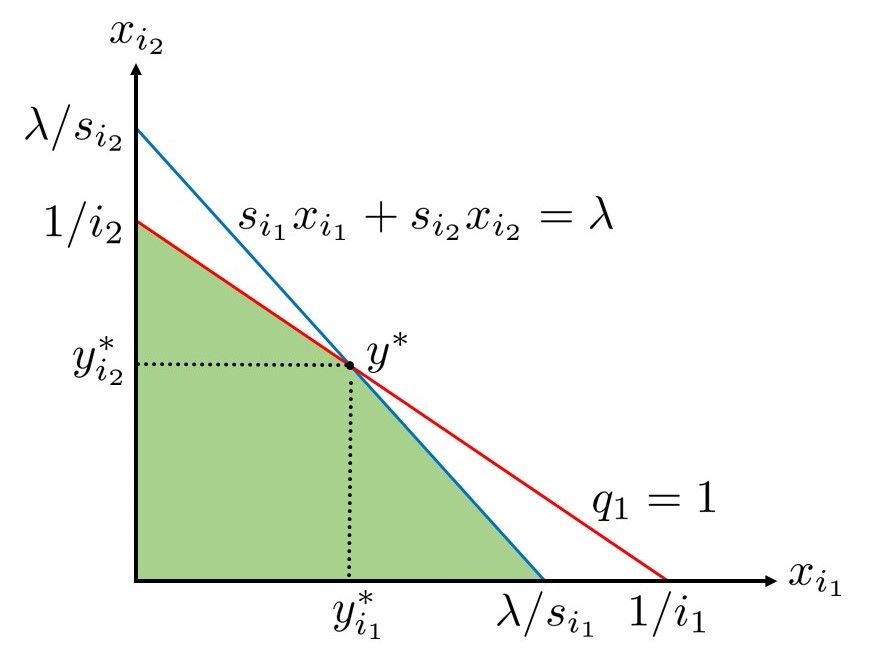
\includegraphics[width=0.5\linewidth]{SSC2.jpg}
\caption{State space of the system collapsing to two dimensions.} 
\label{fig: SSC}
\end{center}
\end{figure}
%
% The first lemma indicates that as the system size increases, the steady-state of the system collapses into at most two dimensions corresponding to the components $i \in I^*$. 

% The second lemma implies that the steady-state probability that the system is in a state where the departure rate exceeds the arrival rate is negligible. To show this, we introduce a secondary Lyapunov function as $V_2(x) = \ind \brac{r > \lambda+\delta}\sum_{i \in [d]} x_i, $
% %
% where $\delta \in (0, 1- \lambda)$ is a constant. Employing Lyapunov drift methods, we show that outside of a suitable compact set, the drift of this Lyapunov function is strictly negative, implying that with a high probability, the function $V_2(x)$ remains within that compact set.

% The third lemma establishes that for large $n$ with high probability the system operates near the intersection of the red line and the green region depicted in Fig~\ref{fig: SSC}.





%
% Given the negligible probability of the system being in a state where the departure rate exceeds the arrival rate, we focus on studying the system under the assumption that the departure rate is below the arrival rate, as described in the third term on the RHS of Inequality~\eqref{eq: three terms to bound}. This assumption corresponds to the system operating within the green region depicted in Figure~\ref{fig: SSC}. This is because, for $|I^*|=2$, the system's state space collapses into a two-dimensional space for large system sizes, as established in Lemma~\ref{lemma: SSC_two dim} while satisfying the system's physical constraints $q_1 \leq 1$. On the other hand, the condition $q_1 = 1- \frac{i_1}{n}$ implies that the system operates close to the red line when $n$ is large. The intersection of the red line and the green region is defined by the conditions $x_{i_1} \leq y_{i_1}^*$ and $x_{i_2} \geq y_{i_2}^*$. Consequently, for sufficiently large $n$, the third term on the RHS of Inequality~\eqref{eq: three terms to bound} should be negative with high probability. In our analysis, however, we could not establish the negativity condition. Nevertheless, we provide an upper bound that is small enough in system size and is presented in the lemma below.

% \begin{figure}
% \begin{center}
% 
\includegraphics[width=0.5\linewidth]{figures/SSC2.jpg}
% \caption{State space of the system collapsing to two dimensions.} 
% \label{fig: SSC}
% \end{center}
% \end{figure}
%

%
% Combining Lemmas~\ref{lemma: generator coupling_sub}--~\ref{lemma: two comp_third bound}, we derive the following corollary.



% \begin{proof}
    
% \end{proof}
%
%Note that when $\lambda  =1 - \beta/n^\alpha \in (0,1)$ for some $\alpha \in [0,1)$ and $\beta >0$, $C_1(\lambda)$, $C_2(\lambda)$, and $C_3(\lambda)$ converge to finite positive constants independent of $\lambda$, as $n \to \infty$. Consequently, if we choose $\delta = o(1)$, the preceding corollary and Lemma~\ref{lemma: SSC_two dim} imply that $\expect{\norm{x - y^*}} \to 0$, showing the convergence in probability of the system state $x$ to $y^*$ as $n \to \infty$.  Therefore, in line with Proposition~\ref{proposition: optimality}, the asymptotic optimality of the $\texttt{greedy}(p^n)$ scheme is established. 




%======================================================================================================================



%======================================================================================================================
\subsection{Proof of Proposition~\ref{prop: full access}}

We first prove the following bound
on the second term on the RHS of~\eqref{eq: first bound for general policy_sub}
after choosing $c_i=1$ for all $i\in I^*$.
\begin{equation}\label{eq: three terms to bound}
   \sum_{i \in I^*} \expect{\brac{x_i - y_i^*} \brac{\lambda A_i(x) - s_i y_i^*}} 
   \leq 
   \frac{2d}{n} 
       +\brac{\frac{2d}{n\lambda}\brac{1+\frac{2}{\delta}} 
       +\frac{2}{\frac{s_{i_1}}{i_1}-\frac{s_{i_2}}{i_2}} \brac{\frac{d}{n}+ \delta}}\ind \brac{|I^*|=2},
  \end{equation}
%
where $\delta \in (0, 1- \lambda)$ is a constant. To prove the above bound, we consider the two cases of $|I^*|=1$ and $|I^*|=2$ separately. For $|I^*| = 1$, recall from Theorem~\ref{thm:optimization} that $y_{i_1}^* = \lambda / s_{i_1}$. Hence, using~\eqref{eq: assign_prob_sub_k=n} and $p_{i_1}^* = s_{i_1} y_{i_1}^* /\lambda$ we obtain
    \begin{align*} 
        \sum_{i \in I^*} \expect{ \brac{x_i - y_i^*} \brac{\lambda A_i(x) - s_i y_i^*}}  
        %\\=  \expect{\frac{i_1}{s_{i_1} y_{i_1}^*} \brac{x_{i_1} - y_{i_1}^*} \brac{\lambda p_{i_1}^* \ind \brac{nq_0 \geq i_1} - s_{i_1} y_{i_1}^*}}
        &=\lambda\expect{\brac{ y_{i_1}^*- x_{i_1} } \ind \brac{q_1 > 1-\frac{i_1}{n}}}\\
        &\leq \lambda \expect{\brac{ y_{i_1}^*- x_{i_1} } \ind \brac{q_1 > 1-\frac{i_1}{n}, y_{i_1}^*\geq x_{i_1}}}\\
        &\leq \lambda \expect{\brac{ i_1 y_{i_1}^*- i_1 x_{i_1} } \ind \brac{q_1 > 1-\frac{i_1}{n}, y_{i_1}^*\geq x_{i_1}}}\\
        &\leq \lambda \expect{\brac{ 1- q_1 + \sum_{i < i_1} ix_i} \ind \brac{q_1 > 1-\frac{i_1}{n}, y_{i_1}^*\geq x_{i_1}}} \leq \frac{2 \lambda i_1}{n}\leq \frac{2 d}{n},
    \end{align*}
%
   % \begin{multline} 
       %\sum_{i \in I^*} \expect{\frac{i}{s_i y_i^*} \brac{x_i - y_i^*} \brac{\lambda A_i(x) - s_i y_i^*}}  
        %=  \expect{i_1 \brac{y_{i_1}^*-x_{i_1} } \ind \brac{nq_0 < i_1}} 
        %\\=\expect{\brac{i_1 y_{i_1}^*-i_1 x_{i_1} } \ind \brac{q_1 \geq 1-\frac{i_1}{n}}}.
    %\end{multline}
%
where the first inequality on the last line follows from the facts that $i_1 y_{i_1}^* \leq \sum_{i \in [d]} i y_i^* \leq 1$ and, for $\abs{I^*}=1$, $i_1 x_{i_1}=q_1 - \sum_{ i < i_1} ix_i$, and the second inequality on the last line follows from
Lemma~\ref{lemma: SSC_two dim} which implies $\sum_{i < i_1} ix_i < i_1/n$.
    
Using a similar line of arguments for the case where $|I^*|=2$, we obtain the following after some simplification.
% \begin{multline}
%    \sum_{i \in I^*} \expect{\frac{i}{s_i y_i^*} \brac{x_i - y_i^*} \brac{\lambda A_i(x) - s_i y_i^*}} 
%      \\= \expect{i_1 \ind\brac{q_1 \geq 1- \frac{i_1}{n}} \brac{y_{i_1}^* - x_{i_1}}}
%     + \expect{i_2 \ind\brac{q_1 > 1- \frac{i_2}{n}} \brac{y_{i_2}^* - x_{i_2}}}
%    \\ + \expect{\frac{i_1 \lambda}{s_{i_1} y_{i_1}^*} \ind \brac{q_1 =1 - \frac{i_1}{n}}\brac{x_{i_1} - y_{i_1}^*}}.
% \end{multline}
% %
% We can rewrite the above equation as 
\begin{align}    
   \sum_{i \in I^*} \expect{\brac{x_i - y_i^*} \brac{\lambda A_i(x) - s_i y_i^*}} 
    & \leq \expect{ \ind\brac{q_1 > 1- \frac{i_1}{n}, y_{i}^*\geq x_i, \forall i \in I^*} \brac{1-q_1+\sum_{i < i_1} i x_i}} \label{eq: first term_sub}
    \\&+ \expect{\ind \brac{q_1 =1 - \frac{i_1}{n}}\brac{(x_{i_1} - y_{i_1}^*)+(y_{i_2}^* - x_{i_2})}}\label{eq: third term_sub}.
\end{align}
%
Expression~\eqref{eq: first term_sub} can be bounded by $2d/n$ as before.
%
To bound \eqref{eq: third term_sub}, we decompose it as follows.
\begin{align} 
    \eqref{eq: third term_sub}
     & = \mathbb{E}\biggl[\ind\brac{q_1 = 1- \frac{i_1}{n}, r > \lambda + \delta} 
    \brac{(x_{i_1} - y_{i_1}^*)+(y_{i_2}^* - x_{i_2})}\biggr]\label{eq: third term_case1_sub}
    \\& +\mathbb{E}\biggl[\ind\brac{q_1 = 1- \frac{i_1}{n}, r \leq \lambda + \delta} 
   \brac{(x_{i_1} - y_{i_1}^*)+(y_{i_2}^* - x_{i_2})}\biggr],\label{eq: bound on third term_case2_sub}
\end{align}
%
where $\delta \in (0 , 1- \lambda)$ is a constant. Now, we have
\begin{equation}
   \eqref{eq: third term_case1_sub}
    \leq 2 \mathbb{P}\brac{ r > \lambda + \delta} \leq \frac{2s_d}{n\lambda}\brac{1+\frac{2}{\delta}}\leq \frac{2d}{n\lambda}\brac{1+\frac{2}{\delta}},
\end{equation}
%
where the second inequality follows from Lemma~\ref{lemma: second Lyapunov function,sublinear} by choosing $\kappa=1/n$ and the last inequality follows from $s_d \leq d$. Finally, \eqref{eq: bound on third term_case2_sub} can be bounded using Lemma~\ref{lemma: two comp_third bound} and noting that 
%$i_1.i_2\geq 1$ and 
$s_{i_1}+s_{i_2}\leq 2d$ to complete the proof of~\eqref{eq: three terms to bound}.

Now to complete the proof of Proposition~\ref{prop: full access}, we note from Lemma~\ref{lemma: generator coupling_sub} that for $c_{i_1}=c_{i_2}=1$, the first term on the RHS of~\eqref{eq: first bound for general policy_sub} is bounded by $1/n$.

% The result follows by choosing 
% $c_i = \frac{i}{s_i y_i^*}$ for $i \in I^*$ in Lemma~\ref{lemma: generator coupling_sub}, $\kappa = \frac{1}{n}$ in Lemma~\ref{lemma: second Lyapunov function,sublinear}, and noting that $y^*_{i_1} = \frac{\lambda}{s_{i_1}}$ when $|I^*|=1$.
%======================================================================================================================


%======================================================================================================================


%======================================================================================================================
\subsection{Proof of Theorem~\ref{thm: main thm}} 

We first note the following.
\begin{align}
\expect{\vert \vert x - y^*\vert\vert} &= \expect{\sum_{ i\not\in I^*} \abs{x_i}} + \expect{\sum_{ i\in I^*} \abs{x_i - y^*_i}}\nonumber\\
& \leq \expect{\sum_{ i\not\in I^*} x_i} + \sqrt{2\expect{\sum_{ i\in I^*} \brac{x_i - y^*_i}^2}}\nonumber\\
&\leq \expect{\sum_{ i\not\in I^*} x_i} + \sqrt{2\expect{\sum_{ i\in I^*} s_i \brac{x_i - y^*_i}^2}}\nonumber\\
&\leq \frac{1}{n}+\sqrt{\frac{2+4d}{n}
+\ind\brac{\abs{I^*}=2}2\brac{\frac{2d}{n}\brac{\frac{1}{\lambda}+\frac{1}{\frac{s_{i_1}}{i_1}-\frac{s_{i_2}}{i_2}}}+\frac{4d}{n\lambda\delta}+\frac{2\delta}{\frac{s_{i_1}}{i_1}-\frac{s_{i_2}}{i_2}}}},\nonumber
\end{align}
%
where the first line follows from the definition of the set $I^*$, the second line follows from Jensen's inequality and the fact that $(a+b)^2\leq 2(a^2+b^2)$ for all $a,b\in \mb{R}$, the third line follows from the fact that $s_i \geq 1$ for all $i \in [d]$, and the last line follows from Lemma~\ref{lemma: SSC_two dim} and Proposition~\ref{prop: full access}. We recall that $\delta \in (0,1-\lambda)$.
Hence, when $\lambda$ varies according to $\lambda=1-\beta n^{-\alpha}$, we must choose $\delta \in (0, \beta n^{-\alpha})$. When $\alpha \in (0,1/2)$, choosing $\delta=\beta/2\sqrt{n}$ gives the lowest possible order of $O(1/n^{1/4})$ for the second term in the last inequality above. However, when $\alpha > 1/2$, the same choice of $\delta$ does not work since the condition $\delta \in (0, \beta n^{-\alpha})$ is violated. Hence, we choose $\delta=\beta/2n^{\alpha}$ which gives the order $O(1/n^{(1-\alpha)/2})$ for the second term on the last line. Thus, combining the above bounds we have
\begin{equation}
\expect{\vert \vert x - y^*\vert\vert}=O\brac{\frac{1}{\sqrt{n}}}+\ind\brac{\abs{I^*}=2}O\brac{\frac{1}{n^{\min(1/4,(1-\alpha)/2)}}}.
\end{equation}

%
To derive a bound on the blocking probability, we use the rate conservation law which yields 
\begin{equation}
    \lambda\brac{1- P_b} = \expect{r} = \sum_{i \in [d]} s_i\expect{x_i}.
\end{equation}
Given the non-negativity of $x_i$ for $i\in [d]$, it follows that $\sum_{i \in [d]} s_i x_i \geq \sum_{i \in I^*} s_i x_i$. Thus,
\begin{equation}
    \lambda P_b \leq \expect{\brac{\lambda - \sum_{i \in I^*}s_{i} x_{i}}} = \sum_{i \in I^*}s_{i} \expect{ y_i^* -x_{i}} \leq d \expect{\norm{x-y^*}},
\end{equation}
%
where the equality follows from the fact that $\sum_{ i\in I^*} s_i y_i^* = \lambda$ and the last inequality follows from the fact that $s_i\leq d$ for all $i \in [d]$. Hence, the bound on the blocking probability has the same order as that of $\expect{\norm{x-y^*}}$.


Similarly, for the mean response time of accepted jobs, we use the Little's law to have
\begin{align}
    \lambda \brac{1-P_b} \expect{D}  = \sum_{i \in [d]} \expect{x_i}.
\end{align}
%
%
Furthermore, since $\lambda D^* = \sum_{i \in [d]} y_i^*$, we have 
\begin{align}
    \lambda  (\expect{D}-D^*)=  &\sum_{i\in [d]}\frac{1}{1-P_b}\expect{x_i-y_i^*}+\frac{P_b}{1-P_b}\sum_{i \in [d]}y_i^*.\nonumber
    %\\ \leq \frac{1}{n} + \sum_{i \in I^*} y_i^* + \sqrt{2\sum_{i\in I^*} \expect{\brac{x_i - y_i^*}^2}}
\end{align}
%
Taking absolute value on both sides of the above equation and using the fact that $\sum_{i \in [d]}y_i^* \leq \sum_{i \in [d]}i y_i^* \leq 1$, we have
\begin{equation}
\lambda  \abs{\expect{D}-D^*}\leq  \frac{1}{1-P_b}\expect{\norm{x-y^*}}+\frac{P_b}{1-P_b}.
\end{equation}
%
From the above it follows that $\abs{\expect{D}-D^*}$ is of the same order as $P_b$ and $\expect{\norm{x-y^*}}$.

% and employing Proposition~\ref{prop: full access}, we arrive at
% \begin{equation} \label{eq: delay inequality}
%     \expect{D} \leq \frac{1}{n\lambda \brac{1-P_b}} + \frac{D^*}{1-P_b} + \frac{\sqrt{2 U^\delta}}{\lambda\brac{1-P_b}},
% \end{equation}
% %
% where $U^\delta$ is given in~\eqref{eq: U-delta}. By choosing $\delta$ in a way that~\eqref{eq:U_delta_order} is satisfied,  %and from~\eqref{eq: block_ineq} for $n$ large enough, 
% we get $\expect{D} \leq D^* + O\brac{\frac{1}{n^{\min\brac{1/4, \brac{1-\alpha}/2}}}}$. On the other hand, $D^*$ is the minimum possible value for $\expect{D}$. Combining these two, we arrive at the desired result. This concludes the proof for the case where $|I^*|=2$. 


For the case $|I^*|=1$, we can derive a stronger bound on $\abs{\expect{D}-D^*}$ as follows. From Little's law, we have
\begin{equation}
    \lambda(1-P_b)\expect{D} = \sum_{i \in [d]} \expect{x_i} \leq \frac{1}{n} + \expect{x_{i_1}},
\end{equation}
%
where the inequality follows from Lemma~\ref{lemma: SSC_two dim}. Noting that $D^* = 1/s_{i_1}$ in this case, we have
\begin{equation*}
    \lambda(1-P_b)\expect{D} \leq \frac{1}{n} + D^*\expect{s_{i_1}x_{i_1}} \leq  \frac{1}{n} + D^*\expect{r} =  \frac{1}{n} + D^*\lambda(1-P_b),
\end{equation*}
%
where the second inequality follows from the non-negativity of $x_i$ for $i \in [d]$ and the equality follows from the rate conservation law. Therefore, we have $\expect{D} \leq \frac{1}{n\lambda(1-P_b)} + D^*$. This inequality combined with the fact that $\expect{D} \geq D^*$ gives the desired result.


\section{Heterogeneous Workloads}
\label{sec:het}

Thus far we have only considered systems where all jobs have the same speed-up function. However, our results can be easily generalized to systems with multiple job classes with different speed-up functions. To see this, let us consider a system with $l$ job classes indexed by $j \in [l]$. As before we drop the superscript $\vphantom{\cdot}^{(n)}$ from our notations for brevity. Let class $j$ jobs be parallelizable up to $d_j$ servers with a speed-up function $s_j=(s_{i,j}, i \in [d_j])$. We assume that the speed-up function for each class satisfies properties \eqref{prop:increasing} and \eqref{prop:concavity}. Then, using the same line of arguments as in Section~\ref{sec:lower}, we have that the optimal scheme which tries to minimize the mean execution time of jobs under the constraint of zero blocking must solve the following optimization problem

\begin{equation}
        \begin{aligned}
        & \underset{y=(y_{ij})} {\text{minimize}}
        & & \frac{1}{\lambda}\sum_{i,j} y_{i,j}\\
        & \text{subject to}
        & & \sum_{i \in [d_j]} s_{i,j} y_{i,j} = \frac{\lambda_j}{\mu_j}, \forall j \in [l],\\
        & & &\sum_{i,j} i y_{i,j} \leq 1,\\
        & & &  y_{i,j} \geq 0, \quad \forall j \in [l], i \in [d_j]
        \end{aligned}
        \tag{Q}
    \label{eq:opt_het}
\end{equation}
%
where $y_{i,j}$ denotes the (scaled) expected number of class $j$ jobs occupying $i$ servers in the steady-state; $\lambda_j$ and $\mu_j$ respectively denote the arrival rate and mean inherent job size of class $j$ and $\lambda = \sum_j \lambda_j$. Defining $\rho_j=\lambda_j/\mu_j$, it is easy to see that the above optimization problem is equivalent to finding the fractions $b_j \in [0,1]$, $j \in [l]$,  of servers to reserve for use of class $j$ jobs such that they solve the following optimization problem

\begin{equation}
        \begin{aligned}
        & \underset{b=(b_{j})} {\text{minimize}}
        & & \sum_{j} f_j(b_j)\\
        & \text{subject to}
        & & \sum_{j} b_j \leq 1,\\
        & & &  b_{j} \geq \rho_j, \quad \forall j \in [l],
        \end{aligned}
        \tag{Q1}
    \label{eq:opt_het_outer}
\end{equation}
%
where $f_j:[0,1]\to \mathbb{R}$ for each class $j \in [l]$ is defined as the optimal objective function value of the following single-class problem for class $j$

\begin{equation}
        \begin{aligned}
        & f_j(b):==\underset{y=(y_{i,j}, i\in [d_j])}{\min}
        & & \frac{1}{\lambda}\sum_{i\in [d_j]} y_{i,j}\\
        & \text{subject to}
        & & \sum_{i \in [d_j]} s_{i,j} y_{i,j} = \rho_j, \\
        & & &\sum_{i\in [d_j]} i y_{i,j} \leq b,\\
        & & &  y_{i,j} \geq 0, \quad \forall i \in [d^{(n)}],
        \end{aligned}
        \tag{Q2}
    \label{eq:opt_het_inner}
\end{equation}
%
Note that the single class optimization problem~\eqref{eq:opt_het_inner}  is equivalent to~\eqref{eq:opt} (after re-defining the decision variables as $y_{i,j}/b$). Hence, the function $f_j$ can be computed in closed form using the results of Theorem~\ref{thm:optimization} and plugging this expression in~\eqref{eq:opt_het_outer}, we can compute the optimal fractions $b_j^*$, $j \in [l]$ of servers to reserve for each class. Once the optimal proportion $b_j^*$ of servers to reserve for each class $j$ has been found in this way, the optimal solution $y_{i,j}^*$ of the original problem~\eqref{eq:opt_het} can be found by solving~\eqref{eq:opt_het_inner} with $b$ replaced by $b_j^*$. It is easy to see that when $\sum_j \rho_j < 1$, there exists a feasible solution to~\eqref{eq:opt_het}. Furthermore, using the $\texttt{greedy}(p_j^*)$ scheme with $p_{i,j}^*=s_{i,j}y_{i,j}^*/\rho_j$ within each class $j$ will lead to asymptotic optimality.  The proof of asymptotic optimality remains the same as the single-class case because,  within each class, the structure of the optimal solution (in particular the SSC property which makes the proof of Theorem~\ref{thm: main thm} work) remains the same as given in Theorem~\ref{thm:optimization} and the classes can be treated independently once we have decided to reserve $b_j^*$ fraction of servers for class $j$ jobs for each $j \in [l]$.
%----------------------------------------------------------------------
\section{Numerical Results} \label{section: numerical results}
%----------------------------------------------------------------------
In this section, we present simulation results that validate our analytical findings. %under the assumption of a strictly increasing and concave speed-up function. 
The simulations are conducted $100$ times, each simulating the arrival of the first $5$ million jobs, with a maximum degree of parallelism set at $d^{(n)}=5$. Two types of speed-up functions are considered: linear (where $s_1=1$, $s_2=2$, $s_3=3$, $s_4=4$, $s_5=5$) and sub-linear (where $s_1=1$, $s_2=1.8$, $s_3=2.5$, $s_4=3$, $s_5=3.4$). Various traffic regimes are simulated, including the mean-field regime with $\alpha=0, \beta = 0.2$, Halfin-Whitt regime with $\alpha=1/2, \beta=0.1$, and super-Halfin-Whitt regime with $\alpha=2/3, \beta=0.1$. Furthermore, 
%we analyze system performance metrics under 
two allocation schemes of $\texttt{greedy}(p^{*,(n)})$ and $\texttt{greedy}$, defined in Section~\ref{sec: main results} are considered. %The former scheme is defined in Section~\ref{sec:main-results}, where the number of servers allocated to each job depends on the arrival rate and the speed-up function through probabilities $p^{*,(n)}$. In contrast, the latter scheme allocates all available servers up to $d^{(n)} = 5$ servers to each incoming job regardless of other factors.
%When the speed-up function is linear, the two schemes become identical. Therefore, we specifically study the effect of different allocation schemes when the speed-up function is sub-linear.

Figure~\ref{fig: blocking,probabilistic} depicts the blocking probability of the system. It is evident that with the $\texttt{greedy}(p^{*,(n)})$ scheme, the blocking probability converges to zero as the system size $n$ increases. However, when employing the $\texttt{greedy}$ scheme with the sub-linear speed-up function, the system exhibits a non-zero blocking probability. This observation highlights the consequence of allocating more servers to each job which can result in a persistent non-zero blocking probability. %as discussed at the beginning of this paper.

Moreover, Figure~\ref{fig: response,probabilistic} presents the mean execution time of accepted jobs. Under the $\texttt{greedy}(p^{*,(n)})$ scheme, the mean execution time of accepted jobs converges to $ D^{*,(n)}= \frac{1}{\lambda^{(n)}}\sum_{i \in I^{*,(n)}} y_i^{*,(n)}$, where the optimal solution $y^{*,(n)}$ is given in Theorem~\ref{thm:optimization}. %based on the speed-up function and arrival rate. 
Specifically, when the speed-up function is linear, $y^{*,(n)} = \brac{0,0,0,0,\lambda^{(n)}/s_5}$, resulting in $D^{*,(n)} = 0.2$. For the sub-linear speed-up function, with $\alpha=0$ and $\beta = 0.2$, the optimal solution $y^{*,(n)}$ is given by $\brac{0, 0,0.2,0.1,0}$ and $D^{*,(n)}=0.375$. For all other cases when the speed-up function is sub-linear and $\alpha>0$, it holds that $y^{*,(n)} \to \brac{1, 0, 0, 0, 0}$, and therefore $D^{*,(n)} \to 1$. Furthermore, it is observed that when employing a sub-linear speed-up function and the $\texttt{greedy}$ scheme, the system achieves a lower average execution time compared to the $\texttt{greedy}(p^{*,(n)})$ scheme 
%under the same traffic conditions. 
; however, at the expense of a non-zero blocking probability, indicating that the scheme is no longer asymptotically optimal. %in this scenario.


%In all scenarios, the mean execution time of accepted jobs converges to its minimum value, demonstrating the asymptotic optimality of the $\texttt{greedy}(p^{*,(n)})$ scheme.
\begin{figure}
\subfigure[Blocking probability of the system]{\label{fig: blocking,probabilistic}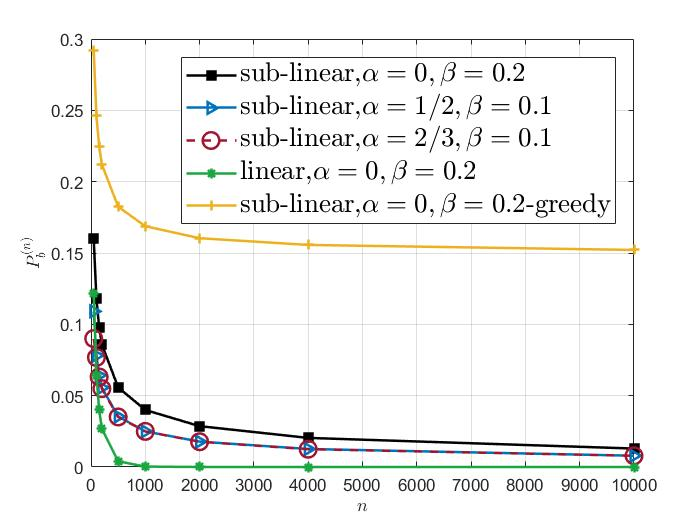
\includegraphics[width=.5\linewidth]{block_P_all.jpg}}\hfill
\subfigure[Mean response time of accepted jobs]{\label{fig: response,probabilistic}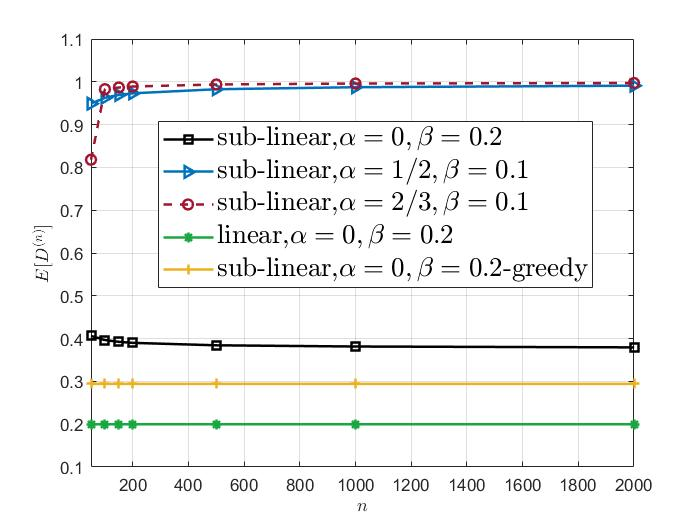
\includegraphics[width=.5\linewidth]{waiting_all.jpg}}
\caption{%The above figure depicts the system performance metrics for different system sizes $n$, when the degree of parallelism is set to $d^{(n)}=5$. Two different speed-up functions are considered where the linear speed-up function satisfies $s_1=1$, $s_2=2$,  $s_3=3$,  $s_4=4$,  $s_5=5$ and the sub-linear speed-up function is given by $s_1=1$, $s_2=1.8$,  $s_3=2.5$,  $s_4=3$,  $s_5=3.4$. Moreover, various traffic conditions are considered to show the applicability and optimality of the values of load parameters (i)$\alpha=0, \beta=0.35$, (ii)$\alpha=0, \beta=0.2$, (iii)$\alpha=0, \beta=0.1$, and (iv)$\alpha=2/3, \beta=5$.
system performance metrics for different system sizes $n$ under $\texttt{greedy}(p^{*,(n)})$ and $\texttt{greedy}$ schemes}
\label{fig: system performance,probabilistic}
\end{figure}

%
%\begin{figure}
%\subfigure[Blocking probability of the system]{\label{fig: blocking,probabilistic}\includegraphics[width=.5\linewidth]{figures/blocking_greedy.jpg}}\hfill
%\subfigure[Mean response time of accepted jobs]{\label{fig: response,probabilistic}\includegraphics[width=.5\linewidth]{figures/mean_Delay_greedy.jpg}}
%\caption{%The above figure depicts the system performance metrics for different system sizes $n$, when the degree of parallelism is set to $d^{(n)}=5$. Two different speed-up functions are considered where the linear speed-up function satisfies $s_1=1$, $s_2=2$,  $s_3=3$,  $s_4=4$,  $s_5=5$ and the sub-linear speed-up function is given by $s_1=1$, $s_2=1.8$,  $s_3=2.5$,  $s_4=3$,  $s_5=3.4$. Moreover, various traffic conditions are considered to show the applicability and optimality of the values of load parameters (i)$\alpha=0, \beta=0.35$, (ii)$\alpha=0, \beta=0.2$, (iii)$\alpha=0, \beta=0.1$, and (iv)$\alpha=2/3, \beta=5$.
%system performance metrics for different system sizes $n$ under the $\texttt{greedy}$ scheme}
%\label{fig:greedy}
%\end{figure}

Finally, we study the insensitivity of the $\texttt{greedy}(p^{*,(n)})$ scheme to the exact distribution of job sizes in Table~\ref{tabel:general size}. We consider the same system parameters %for $d^{(n)}$, the speed-up functions, and the traffic parameters. 
and study a system with $n=4000$ servers, considering exponential (Exp), deterministic (Det), Mixed-Erlang, and Pareto distributions, all with the same unit mean. The Mixed-Erlang distribution includes two exponential phases with probabilities $p_1=0.4$, and $p_2=0.6$. The CDF of the Pareto distribution is given by
$\mathbbm{P} \brac{Y \leq y} = \begin{cases}
     1- \frac{1}{(3y)^{3/2}},\quad &\text{ if } y \geq \frac{1}{3}\\
     0, \quad &\text{otherwise}
\end{cases}$. Results in Table~\ref{tabel:general size} show the system's performance is insensitive to the exact distribution of job lengths.%and remains asymptotically optimal for all job size distributions.

\renewcommand{\arraystretch}{0.7}
\begin{table*}[htbp]
\caption{Performance metrics of a system with $n=4000$ servers under different job size distributions}
\small
\makebox[\textwidth][c]{\begin{tabular}{c|m{3.5em}m{3.5em}m{3.5em}m{3.5em}|m{3.5em}m{3.5em}m{3.5em}m{3.5em}}
\toprule
 &\multicolumn{4}{c|}{Mean Execution Time $\expect{D^{(n)}}$} &  \multicolumn{4}{c}{Blocking Probability $P_b^{(n)}$}\\
\midrule
Inherent Size Distribution & Exp & Det & Mixed Erlang& Pareto&Exp & Det & Mixed Erlang& Pareto\\
\midrule
 %linear speed-up, $\alpha=0, \beta = 0.35$ & $0.2000$ & 0.2000& 0.2000&0.1975& 0& 0& 0&0\\
linear speed-up, $\alpha=0, \beta = 0.2$ &0.2000&0.2000&0.2000&0.1973&0& 0& 0&0 \\
 linear speed-up, $\alpha=1/2, \beta = 0.1$ &0.2000&0.2000&0.2000&0.1970&0.0267&0.0268&0.0267&0.0209 \\
 linear speed-up, $\alpha=2/3, \beta = 0.1$ &0.2000&0.2000&0.2000&0.1971&0.0274&0.0274&0.0274&0.0219  \\
\hline
%sub-linear speed-up, $\alpha=0, \beta = 0.35$ &0.2941&0.2941&0.2941&0.2898&0.0070&0.0070&0.0070&0.0048\\
sub-linear speed-up, $\alpha=0, \beta = 0.2$ &0.3782&0.3782&0.3782&0.3708&0.0204&0.0202&0.0203&0.0149 \\
sub-linear speed-up, $\alpha=1/2, \beta = 0.1$ &0.9930&0.9937&0.9933& 0.9621&0.0126&0.0126&0.0126& 0.0041\\
sub-linear speed-up, $\alpha=2/3, \beta = 0.1$ &0.9976&0.9984&0.9979&0.9669&0.0125&0.0125&0.0125&0.0041 \\
\bottomrule
\end{tabular}
}
\label{tabel:general size}
\end{table*}

%----------------------------------------------------------------------
\section{Conclusion} \label{section: conclusion}
%-------------------------------------------------------------------In this paper, we studied multi-server jobs that can run on a flexible number of servers simultaneously. It was assumed that the speed-up in job execution time was a strictly increasing and concave function of the number of servers processing it. Our objective was to devise a server allocation scheme minimizing the mean execution time while ensuring zero blocking probability. To achieve this, we first analyzed the optimal system state and showed that it is at most two-dimensional. Then, we introduced the $\texttt{greedy}(p^{*,(n)})$ scheme, allocating servers to each job by probabilities that corresponded directly to the optimal system state. We showed that as the system size approaches infinity, this scheme achieves zero blocking probability and the minimum average execution time of jobs.

The present paper opens up many directions for future research. One immediate problem to address is to analytically establish the insensitivity of the system operating under the $\texttt{greedy}(p^{*,(n)})$ scheme. This will require studying the system under more general distributions. Another interesting direction to pursue is to consider multi-phase jobs with each phase having a different speed-up function. Obtaining optimal schemes for such a system in the stochastic setting is a challenging open problem. Furthermore, our scheme requires the knowledge of the arrival rate and the speed-up functions of jobs to make optimal server allocations. Deriving schemes which can automatically learn these parameters will be an interesting problem to consider.
%
%The $\texttt{greedy}(p^{*,(n)})$ scheme depends on knowing the arrival rate and the speed-up function. Future research may study adaptive policies identifying arrival rate regions based on observed blockings, eliminating the need for precise system parameter knowledge.%Analyzing these adaptive policies presents intriguing insights into system performance under such strategies.
\bibliographystyle{unsrt}
\bibliography{MobiRef_trunc3.bib}
\appendix
%\vspace{-1 mm}

\section{Proof of Proposition~\ref{proposition: optimality}}
\label{proof:optimality}
First, we note that for $\lambda^{(n)} \in [0,1]$, the $d^{(n)}$-dimensional vector $(\lambda^{(n)},0,\ldots,0)$ is a feasible solution of~\eqref{eq:opt}. Furthermore, by comparing the first two constraints of~\eqref{eq:opt}, it is clear that for there to be a feasible solution to~\eqref{eq:opt}, we must have $\lambda^{(n)} \leq 1$ since by~\eqref{eq:concave} we have $s_i \leq i$ for all $i \in [d^{(n)}]$.

% The rate conservation principle and Little's law respectively yield    
% \begin{align}
% \expect{r(x^n)}=&\expect{\sum_{i \in [d^n]} s_i x_i^n}=\lambda^n (1-P_b^n), \label{eq:rate_conservation_sub}
% \\
%  \expect{\sum_{i\in [d^n]}x_i^n}&=\lambda^n(1-P_b^n)\expect{D^n}  \label{eq:little_sub}.
% \end{align}
% %
% Furthermore, the system state must be such that the total number of busy servers is at most $n$ which gives
% $$\expect{q_1^n}=\expect{q_1(x^n)}=\sum_{i \in [d^n]} i \expect{x_i^n} \in [0,1].$$
Subtracting~\eqref{eq:rate_consevation} from the first constraint of problem~\eqref{eq:opt}
we obtain $$r(y^{*,(n)})-\expect{r^{(n)}}=\sum_{i\in [d^{(n)}]}s_i \expect{y^{*,(n)}_i-x_i^{(n)}}=\lambda^{(n)} P_b^{(n)}.$$
Hence, taking the absolute values of both sides, using the triangle inequality, and the fact that $s_i \leq d^{(n)}$ for all $i \in [d^{(n)}]$, we obtain $\lambda^{(n)} P_b^{(n)} \leq d^{(n)} \expect{\norm{x^{(n)}-y^{*,(n)}}}$.
Thus, if $\expect{\norm{x^{(n)}-y^{*,(n)}}} \to 0$ for a scheme, then $P_b^{(n)}\to 0$ for the same scheme. Now, we note that $\lambda^{(n)}\expect{D^{(n)}}=\frac{\sum_{i \in [d^{(n)}]}\expect{x_i^{(n)}}}{1-P_b^{(n)}}$ and ${\lambda^{(n)}}{D^{*,(n)}}={\sum_{i \in [d^{(n)}]}{y_i^{*,(n)}}}$. 
Hence, we have
$\abs{\lambda^{(n)}(\expect{D^{(n)}}-D^{*,(n)})}\leq \frac{1}{1-P_b^{(n)}}\expect{\norm{x^{(n)}-y^{*,(n)}}}+\frac{P_b^{(n)}}{1-P_b^{(n)}}.$ The desired result follows from the above inequality since  $P_b^{(n)}\to 0$ and $\expect{\norm{x^{(n)}-y^{*,(n)}}} \to 0$.
% taking the limit of~\eqref{eq:little_sub} as $n \to \infty$ and using the facts $P_b^n \to 0$ and $\expect{x_i^n} \to y^{*,n}$, we obtain $\expect{D^n} \to \frac{1}{\lambda^n}\sum_{i \in [d^n]}x_i^*$. Since, $y^{*,n}$ is an optimal solution of~\eqref{eq:opt}, this shows that the steady-state mean execution time of jobs $\expect{D^n}$ approaches to its minimum value as $n \to \infty$. 



\section{Proof of Theorem~\ref{thm:optimization}}
\label{proof: optimization proposition}

To simplify notations, we drop the superscript $\vphantom{\cdot}^n$ from all the notations used in the proof. The Lagrangian function for~\eqref{eq:opt} is given by

\begin{equation*}
    \mathcal{L}\brac{y,\nu, \theta_0, \theta_1, \ldots, \theta_d} = \frac{1}{\lambda}\sum_{i \in [d]} y_i + \nu \brac{\sum_{i \in [d]} s_i y_i - \lambda}+ \theta_0 \brac{\sum_{i \in [d]} i y_i -1} - \sum_{i \in [d]} \theta_i y_i,    
\end{equation*}
%
where $\nu \in \mb R$, $\theta_0 \geq 0$, and $\theta_i \geq 0$, $i\in [d]$ denote the Lagrange multipliers associated with the equality constraint, the first inequality constraint and the non-negativity constraints of~\eqref{eq:opt}, respectively. Slater's condition for strong duality holds since $y = \brac{\lambda, 0, \ldots, 0}$ is a feasible solution for all $\lambda \in (0,1]$. Consequently, any primal optimal solution $y = \brac{y_1, \ldots, y_d}$ and dual optimal solution $\brac{\nu, \theta_0, \theta_1,\ldots,\theta_d}$ must satisfy Karush-Kuhn-Tucker (KKT) conditions given below.

\begin{align}
    &\frac{\partial{\mathcal{L}}}{\partial{y_i}} = \frac{1}{\lambda} + \nu s_i + \theta_0 i - \theta_i =0, \forall i \in [d],  \label{eq: zero derivative}
    \\ &\theta_0 \geq 0, \quad \theta_i \geq 0, \forall i \in [d], \quad   \label{eq: dual feas}
    \\& \theta_0 \brac{\sum_{i \in [d]} i y_i -1}=0, \quad \theta_i y_i=0, \forall i \in[d], \quad \label{eq: slackness}
    \\& \sum_{i \in [d]} s_i y_i  = \lambda, \quad \sum_{i \in [d]} i y_i \leq 1, \quad y_i \geq 0, \forall i \in [d]. \quad  \label{eq: primal feas}
\end{align}
%
From the primal feasibility constraint  $\sum_{i \in [d]} s_i y_i = \lambda >0$ (in \eqref{eq: primal feas}), it follows that $y_i>0$ for at least one $i \in [d]$. The complementary slackness condition $\theta_i y_i =0$ (in \eqref{eq: slackness}) requires  $\theta_i=0$ if $y_i >0$. Let $\theta_i =0$ (or, equivalently, $y_i > 0$) for $K \geq 1$ distinct indices of $i \in \{i_1,i_2,\ldots,i_K\} \subseteq [d]$ with $i_1 < i_2 < \ldots <i_K$, and $\theta_i >0$ for all other indices. Hence, by~\eqref{eq: zero derivative} we have

\begin{align} \label{eq: zero thetai}
    \frac{1}{\lambda}+ \nu s_{i_k} + \theta_0 i_k = \theta_{i_k} = 0, \quad \forall k \in [K].
\end{align}
%

We consider two cases: one where $\theta_i = 0$ for at least two distinct indices of $i$, i.e., $K \geq 2$, and the other where $\theta_i = 0$ for a single index $i$, i.e., $K=1$. 

\begin{enumerate}
   \item \textbf{The $K\geq 2$ case:} In this case, we must have $\nu\neq 0$ as $\nu=0$ implies by~\eqref{eq: zero thetai} that $\theta_0=-1/i_k \lambda$ for at least two distinct values of $i_k$ which is not possible. Hence, $\nu\neq 0$ and this by~\eqref{eq: zero thetai} implies
\begin{equation} \label{eq: theta0 / nu}
    -\frac{\theta_0}{\nu} = \frac{s_{i_{k_2}} - s_{i_{k_1}}}{i_{k_2} - i_{k_1}}, \quad \forall k_1 <k_2,~ k_1, k_2 \in [K].
\end{equation}
%
 We show that all indices $\{i_1,i_2,\ldots,i_K\}$ must be consecutive, i.e., $i_{k+1}=i_k+1$ for all $k \in [K-1]$. Assume it is not true. Therefore, $i_k + 1 < i_{k+1}$ for some $ k \in [K]$. Then, the interval $\brac{i_k, i_{k+1}}$ contains at least one index $i \in [d]$. Furthermore, by definition of the set of indices $\{i_1,i_2,\ldots,i_K\}$, for any $i \in \brac{i_k, i_{k+1}}$, we must have $\theta_i >0$. Consequently, using~\eqref{eq: zero derivative} for $i$ and $i_k$ we have

\begin{align}
   &\frac{1}{\lambda} + \nu s_i + \theta_0 i  = \theta_i >0, \quad \forall i \in \brac{i_k, i_{k+1}}.
\end{align}
Using the above and~\eqref{eq: zero thetai} we have
\begin{equation}
    -\frac{\theta_0}{\nu} > \frac{s_i - s_{i_k}}{i - i_k},\quad \forall i \in \brac{i_k, i_{k+1}}.
\end{equation}
%
Combined with~\eqref{eq: theta0 / nu} the above yields

\begin{equation}
    \frac{s_{i_{k+1}} - s_{i_k}}{i_{k+1} - i_k} >\frac{s_i - s_{i_k}}{i - i_k}, \quad \forall i \in \brac{i_k, i_{k+1}},
\end{equation}
%
which is equivalent to

\begin{equation}
    s_i < \brac{1- \frac{i - i_k}{i_{k+1}-i_k}} s_{i_k} + \frac{i-i_k}{i_{k+1} - i_k} s_{i_{k+1}}, 
\end{equation}
%
for all $i \in \brac{i_k, i_{k+1}}$. Since $\frac{i - i_k}{i_{k+1}-i_k} \in (0,1)$ for any $i \in \brac{i_k, i_{k+1}}$, the above inequality violates the concavity of the speed-up function. Therefore, we conclude that

\begin{equation} \label{eq: consecutive index}
    i_{k+1} = i_k +1, \quad \forall k \in [K-1].
\end{equation}
%
Applying the above in~\eqref{eq: theta0 / nu}, we conclude that 

\begin{equation} \label{eq: constant diff Delta}
    s_{i_{k+1}} - s_{i_k} = -\frac{\theta_0}{\nu}, \quad \forall k \in [K-1],
\end{equation}
%
This implies that $\theta_0 >0$ as otherwise \eqref{eq: constant diff Delta} leads to $s_{i_{k+1}}=s_{i_k}$ for all $k \in [K-1]$, contradicting~\eqref{eq:increasing}. 
For simplicity, we shall denote the ratio $-\theta_0/\nu$ by $\Delta$. Note that by~\eqref{eq: zero thetai} we have
 \begin{equation}
            s_{i_K} - \Delta i_K = s_{i_{K-1}} - \Delta i_{K-1} = \ldots = s_{i_1} - \Delta i_1.
            \label{eq:identity}
\end{equation}

   
   Since $\theta_0>0$, by the complementary slackness condition $\theta_0 \brac{\sum_{i \in [d]} i y_i -1 }=0$, we obtain $\sum_{i \in [d]} i y_i =1$. Further, since $y_i$ is non-zero only for $i \in \{ i_1, i_2, \ldots, i_K \}$, we have

   \begin{align}
       \sum_{k=1}^K s_{i_k} y_{i_k} &= \lambda,\label{eq:rate}
       \\\sum_{k=1}^K i_k y_{i_k} &= 1.\label{eq:capacity}
   \end{align}
    %
   However, from~\eqref{eq: consecutive index} and \eqref{eq: constant diff Delta}, we have $i_k = i_1 + (k-1)$ and $s_{i_k} = s_{i_1} +  (k-1)\Delta$ for any $k \in [K]$. As a result, we obtain

   % \begin{align}
   %     s_{i_1}\sum_{k=1}^K y_{i_k} + \Delta \sum_{k=2}^K (k-1)y_{i_k}&= \lambda,
   %     \\ i_1 \sum_{k=1}^K y_{i_k} + \sum_{k=2}^K (k-1)y_{i_k} &= 1.
   % \end{align}

   %  Solving these equations results in

    \begin{align}
        \brac{s_{i_1} - \Delta i_1} \sum_{k=1}^K y_{i_k} &= \lambda - \Delta,
        \label{eq: sum first K}\\ \sum_{k=1}^K (k-1) y_{i_k} &= 1- i_1 \sum_{k=1}^K y_{i_k}. \label{eq: sum first K scaled}
    \end{align}

    We note that $\Delta = \lambda$ is not possible since it implies by~\eqref{eq: sum first K} that $s_{i_1}-\Delta i_1 =0$. But, by~\eqref{eq:identity} this implies $\frac{s_{i_k}}{i_k} = \Delta = \lambda$, for all $k \in [K]$ substituting which in~\eqref{eq: zero thetai} yields
%
        $$\nu \lambda + \theta_0 = -\frac{1}{\lambda i_k}, \quad \forall k \in [K].$$
%
    However, the above cannot hold for more than one distinct values of $i_k$. Hence, $\Delta \neq \lambda$ which by~\eqref{eq: sum first K}-\eqref{eq: sum first K scaled} implies that

        \begin{align}
            \sum_{k=1}^K y_{i_k} &= \frac{\lambda - \Delta}{s_{i_1} - \Delta i_1}, \label{eq: first K sum subcase2}
            \\
            \sum_{k=2}^K (k-1) y_{i_k} &= 1- i_1\sum_{k=1}^K y_{i_k} = \frac{s_{i_1}-\lambda i_1}{s_{i_1}-\Delta i_1}. \label{eq: first K-1 sum subcase2}
        \end{align}

        We now claim that $s_{i_1}-\Delta i_{1} > 0$ and therefore by~\eqref{eq:identity} $s_{i_k}-\Delta i_k >0$ for all $k \in [K]$.
        Assume that the above is not true, i.e., $s_{i_k}-\Delta i_k < 0$ for all $k \in [K]$. Then, by~\eqref{eq: constant diff Delta} we obtain
        \begin{align}
            \frac{s_{i_k}}{i_k} < \Delta  = s_{i_{k+1}} - s_{i_k}, \quad \forall k \in [K-1].
            \label{eq:strict}
        \end{align}
        %
        But since $i_{k+1}=i_k+1$ for all $k \in [K-1]$, the above implies $s_{i_{k}}/i_k < s_{i_{k+1}}/i_{k+1}$ which contradicts~\eqref{eq:concave}. Hence, We conclude that $s_{i_k}-\Delta i_k >0$ for all $k \in [K]$. This shows that the direction of inequality in~\eqref{eq:strict} should be reversed and therefore the following must hold.
        \begin{equation}
            \frac{s_{i_1}}{i_1} > \frac{s_{i_2}}{i_2} > \ldots > \frac{s_{i_K}}{i_K}.
        \end{equation}
        %
        But the above implies that $$\sum_{k\in [K]} s_{i_k} y_{i_k}=\sum_{k\in [K]} (s_{i_k}/i_k) i_k y_{i_k} \in \brac{\frac{s_{i_K}}{i_K},\frac{s_{i_1}}{i_1}}$$ since $\sum_{k \in [K]} i_k y_{i_k}=1$ by~\eqref{eq:capacity}.
        Hence, by~\eqref{eq:rate} we must have
        $\lambda \in \brac{\frac{s_{i_K}}{i_K},\frac{s_{i_1}}{i_1}}$.
        Hence, to summarize, we have shown the following: for $K\geq 2$ if there exists $\{i_1,i_2,\ldots,i_K\}\subseteq[d]$ such that
        \begin{itemize}
            \item $i_{k+1}=i_k+1, \forall k\in [K-1]$,
            \item $s_{i_{k+1}}-s_{i_k} =\Delta $ for some  constant $\Delta >0$ and all $k \in [K-1]$,
            \item $s_{i_{k}}/i_k > s_{i_{k+1}}/i_{k+1}, \forall k \in [K-1]$,
            \item and $\lambda \in \brac{\frac{s_{i_K}}{i_K},\frac{s_{i_1}}{i_1}}$,
        \end{itemize}
        %
        then any 
        $y\in \mathbb{R}^d_+$ which satisfies~\eqref{eq: first K sum subcase2},~\eqref{eq: first K-1 sum subcase2},  and $y_i=0$ for all $i\notin \{i_1,i_2,\ldots,i_K\}$ is a primal optimal solution of~\eqref{eq:opt}. In particular,
        \begin{align*}
            y_{i_k}&=\frac{\frac{1}{i_k}\brac{\lambda-\frac{s_{i_{k+1}}}{i_{k+1}}}}{\frac{s_{i_k}}{i_k}-\frac{s_{i_{k+1}}}{i_{k+1}}}, \\ 
            y_{i_{k+1}}&=\frac{\frac{1}{i_{k+1}}\brac{\frac{s_{{i_k}}}{i_k}-\lambda}}{\frac{s_{i_k}}{i_k}-\frac{s_{i_{k+1}}}{i_{k+1}}},\\
            y_i&=0, \forall i \notin \{i_{k},i_{k+1}\}.
        \end{align*}
        constitutes one such optimal solution. Furthermore, when $K=2$, the above is the unique optimal solution. This establishes the last part of Theorem~\ref{thm:optimization}.
     

        
    
    \item \textbf{The $K=1$ case:} Let $i_1 \in [d]$ be the only index for which $\theta_{i_1} =0$. Therefore, $\theta_i >0$ for all $i \neq i_1$ and the complementary slackness condition $\theta_i y_i=0$ in~\eqref{eq: slackness} implies $y_{i}=0$ for all $i \not= i_1$. As a result, from primal feasibility constraint $\sum_{i \in [d]} s_{i} y_i = \lambda$, we obtain
    \begin{align*}
        y_{i_1} = \frac{\lambda}{s_{i_1}},\quad y_{i} = 0,~ \forall i \not = i_1.
    \end{align*}

    Two sub-cases emerge based on whether $\lambda < s_{i_1} / i_1$ or $\lambda = s_{i_1} / i_1$.
    \begin{itemize}
        \item Sub-case $1$, $\lambda< s_{i_1} / i_1$: In this sub-case,  $\sum_{i \in [d]} i y_i  = i_1 y_{i_1}=\frac{i_1\lambda}{s_{i_1}}<1$ which implies $\theta_0 = 0$. Consequently, from~\eqref{eq: zero derivative} we obtain
    \begin{align*}
        &1/\lambda+ \nu s_{i_1} = \theta_{i_1}=0
        \\ &1/\lambda+ \nu s_i = \theta_i >0, \quad\forall i \not= i_1.
    \end{align*}
    % The above relationships imply $s_i < s_{i_1}$ for all $i \not= i_1$. Given~\eqref{eq:increasing}, it follows that $i_1=d$ and, therefore, $y=\brac{0,\ldots,0,\lambda/s_d}$. This completes the proof of the first part of Theorem~\ref{thm:optimization}.

    \item Sub-case $2$, $\lambda =  s_{i_1} / i_1$: In this sub-case, the only non-zero component of $y$ is given by 
    $$
    y_{i_1}  =  \frac{\lambda}{s_{i_1}} = \frac{1}{i_1}.$$
    %
    Hence, the objective function becomes $1/\lambda i_1$. Therefore, if there exists multiple indices $i \in [d]$ for which $\lambda=s_i/i$, then the objective function will be minimized only if we choose $i_1 = \max \{i: \lambda   = s_{i} / i \}$. 
     \end{itemize}
     The above two sub-cases together completes the proof of the first two parts of Theorem~\ref{thm:optimization}.
\end{enumerate}
%

\section{Proof of Lemma~\ref{lemma: SSC_two dim}}

To prove the lemma, it is sufficient to assume the system starts at a state where $\sum_{ i\not\in I^*}x_i=0$ since, due to ergodicity, starting from any other state the system will reach a state satisfying the above condition in a finite time with probability one. Now, if the system starts at a state satisfying $\sum_{ i\not\in I^*}x_i=0$, then the $\texttt{greedy}(p^*)$ scheme will keep allocating each incoming job either $i_1$ or $i_2$ free servers until the number of free servers in the system falls strictly below $i_1$. Until this point, the value of $x_{i}$ for $i \notin I^*$ will remain zero. Once the number of free servers in the system falls strictly below $i_1$, the next arrival increases $\sum_{i < i_1} x_i$ from zero to at most $1/n$. This job is referred to as the {\em tagged job}. If, upon arrival of the tagged job, $\sum_{i < i_1} x_i$ increases to $1/n$, then the system must have become fully occupied after the arrival of the tagged job. This is because of the fact that the $\texttt{greedy}(p^*)$ scheme allocates all available servers to an incoming job if the number of available servers goes below $i_1$. Hence, until the tagged job leaves the system, subsequent arrivals either find the system fully busy (and are therefore blocked) or find at least $i_1$ servers available (which occurs if a job occupying $i_1$ or $i_2$ servers departs before the arrival occurs and the tagged job leaves the system). In either case, the sum $\sum_{i < i_1} x_i$ remains constant at $1/n$ until the tagged job departs. Upon the departure of the tagged job, $\sum_{i < i_1} x_i$ returns to zero. From this point onward we can apply the same chain of arguments as above. This shows that $\sum_{i < i_1} x_i$ never exceeds $1/n$. Furthermore, at all times, there is no increase in the number of components $x_i$ for $i > i_2$ because under the $\texttt{greedy}(p^*)$ the probability of a job being allocated more than $i_2$ servers is zero.


\section{Proof of Lemma~\ref{lemma: second Lyapunov function,sublinear}}


Assume that the system is in a state where $V_2(x)  \geq \kappa$ for some $\kappa>0$. By definition of $V_2$, this can only happen when $r > \lambda+\delta$. An arrival can only increase the value of $r$ and a departure can decrease it by at most $s_d/n \leq d/n$. Hence, when $V_2(x)  \geq \kappa > 0$, $d=o(n)$, and $n$ is sufficiently large, the value of $r$ after an arrival or a departure  still remains above $\lambda+\delta$.
% \begin{equation}\label{eq: condition1_sub}
%         \ind\brac{r > \lambda+\delta} =1 \text{, and }
%         r> \lambda+\delta.
%     \end{equation}
%
Hence, given $V_2(x)  \geq \kappa$, the drift of the function $V_2(x)$ under $G$ for sufficiently large $n$ satisfies
\begin{align}
    GV_2(x) = \lambda \sum_{i \in [d]} A_i(x)  - \sum_{i \in [d]} s_ix_i
     \leq  \lambda - r 
    < -\delta,
\end{align}
where the second inequality follows from the fact that $r > \lambda +\delta$ (since $V_2(x)  \geq \kappa$). %This shows that outside of the set $\{x:V_2(x) < \kappa, \kappa>0\}$, the function has a negative drift. 
We now apply Lemma~4 of~\cite{lei_ying_2020_Stein} %, as recalled in Appendix~\ref{appendix: tail_bound},
to conclude that
\begin{align} \label{eq: expect_v2}
     \expect{V_2(x)} \leq  \kappa+\frac{2}{ n\delta}.
\end{align}
This completes the proof of the first part of the lemma. For the second part, note that
\begin{align*}
   \lambda \mathbbm{P}\brac{r > \lambda + \delta}  &=  \lambda \expect{\ind \brac{r > \lambda + \delta}}
  \leq \expect{\ind \brac{r > \lambda + \delta} r} 
   \nonumber\\& \leq s_d \expect{\ind \brac{r > \lambda + \delta} \sum_{i \in [d]}x_i}
   \leq  s_d\brac{\kappa+\frac{2}{ n\delta}},
\end{align*}
%
where the first inequality in the second line follows since $r = \sum_{i \in [d]} s_i x_i \leq s_d \sum_{i\in[d]} x_i$, and the last inequality follows from the definition of $V_2(x)$ and~\eqref{eq: expect_v2}. This completes the proof.

\section{Proof of Lemma~\ref{lemma: two comp_third bound}}

Given that $|I^*|=2$, $q_1=1-i_1/n$, and $r \leq \lambda +\delta$,  we have the following using the definitions of $q_1$ and $r$.
\begin{align}
    i_1 x_{i_1} + i_2 x_{i_2} +\sum_{i < i_1} ix_i&= 1 - \frac{i_1}{n},\label{eq:elim1}
    \\s_{i_1}x_{i_1} + s_{i_2}x_{i_2} +\sum_{i <i_1}s_ix_i& \leq \lambda + \delta.
    \label{eq:elim2}
\end{align}
%
By eliminating $x_{i_2}$ from the above we obtain
\begin{align}
    %&x_{i_2} \geq \frac{1}{i_2} - 2\frac{i_1}{i_2n } - \frac{i_1 x_{i_1}}{i_2},
    {i_1}x_{i_1} \brac{\frac{s_{i_1}}{i_1}-\frac{s_{i_2}}{i_2}} - (\lambda -\frac{s_{i_2}}{i_2}) &\leq \delta + \frac{i_1 s_{i_2}}{n i_2}+\sum_{i < i_1} \brac{\frac{s_{i_2}}{i_2}-\frac{s_{i}}{i}} ix_i\\
    &\leq \delta + \frac{i_1 s_{i_2}}{n i_2},
\end{align}
%
where the last line follows since $\frac{s_{i_2}}{i_2}\leq \frac{s_i}{i}$ for all $i <i_1$ by~\eqref{eq:concave}.
%
% We rewrite the above inequality as
% \begin{equation}
%     i_1x_{i_1} \brac{\frac{s_{i_1}}{i_1} - \frac{s_{i_2}}{i_2}} 
%  - \brac{\lambda - \frac{s_{i_2}}{i_2}}  \leq 2\frac{i_1s_{i_2}}{i_2n } + \delta- \sum_{i <i_1} s_i x_i.
% \end{equation}
%
Now, using $y_{i_1}^* = \frac{\frac{1}{i_1} \brac{ \lambda- \frac{s_{i_2}}{i_2}}}{\frac{s_{i_1}}{i_1}-\frac{s_{i_2}}{i_2}}$ we obtain
\begin{equation}
(x_{i_1}-y_{i_1}^*)\leq \frac{\frac{\delta}{i_1} + \frac{s_{i_2}}{n i_2}}{\frac{s_{i_1}}{i_1}-\frac{s_{i_2}}{i_2}}.
\end{equation}
%
Similarly, eliminating $x_{i_1}$ from~\eqref{eq:elim1} and~\eqref{eq:elim2} we obtain
\begin{equation}
(y_{i_2}^*-x_{i_2})\leq \frac{\frac{\delta}{i_2} + \frac{s_{i_1}}{n i_2}}{\frac{s_{i_1}}{i_1}-\frac{s_{i_2}}{i_2}}.
\end{equation}
%
Combining the above two we obtain the result of the lemma.

\end{document}